% This is the default LaTeX template (default-1.17.0.2.tex) from the RMarkdown package, from:
% https://github.com/rstudio/rmarkdown/blob/master/inst/rmd/latex/default-1.17.0.2.tex
%
% New additions to the template are marked with "LCR"

%\documentclass[11pt,spanish,]{book} %LCR
 % if not, force the oneside and a4paper options, which seem to be the only reasonable defaults
\documentclass[11pt,spanish,a4paper,oneside,]{book} %LCR

\usepackage{lmodern}
\usepackage{amssymb,amsmath}
\usepackage{ifxetex,ifluatex}
\usepackage{fixltx2e} % provides \textsubscript
\ifnum 0\ifxetex 1\fi\ifluatex 1\fi=0 % if pdftex
  \usepackage[T1]{fontenc}
  \usepackage[utf8]{inputenc}
\else % if luatex or xelatex
  \ifxetex
    \usepackage{mathspec}
  \else
    \usepackage{fontspec}
  \fi
  \defaultfontfeatures{Ligatures=TeX,Scale=MatchLowercase}
\fi
% use upquote if available, for straight quotes in verbatim environments
\IfFileExists{upquote.sty}{\usepackage{upquote}}{}
% use microtype if available
\IfFileExists{microtype.sty}{%
\usepackage{microtype}
\UseMicrotypeSet[protrusion]{basicmath} % disable protrusion for tt fonts
}{}

 %LCR
\usepackage{hyperref}
\PassOptionsToPackage{usenames,dvipsnames}{color} % color is loaded by hyperref
\hypersetup{unicode=true,
            pdftitle={Evaluación de la selección genómica de un solo paso en arroz},
            pdfauthor={Jorge Leonardo López Martínez},
            colorlinks=true,
            linkcolor=cyan,
            citecolor=Blue,
            urlcolor=cyan,
            breaklinks=true}
\urlstyle{same}  % don't use monospace font for urls
\ifnum 0\ifxetex 1\fi\ifluatex 1\fi=0 % if pdftex
  \usepackage[shorthands=off,main=spanish]{babel}
\else
\usepackage{polyglossia}
  \setmainlanguage{spanish}
  % Tabla en lugar de cuadro
  \gappto\captionsspanish{\renewcommand{\tablename}{Tabla}  
          \renewcommand{\listtablename}{Índice de tablas}}
\else
  \usepackage[spanish,es-tabla]{babel}
\fi
\usepackage{color}
\usepackage{fancyvrb}
\newcommand{\VerbBar}{|}
\newcommand{\VERB}{\Verb[commandchars=\\\{\}]}
\DefineVerbatimEnvironment{Highlighting}{Verbatim}{commandchars=\\\{\}}
% Add ',fontsize=\small' for more characters per line
\usepackage{framed}
\definecolor{shadecolor}{RGB}{248,248,248}
\newenvironment{Shaded}{\begin{snugshade}}{\end{snugshade}}
\newcommand{\AlertTok}[1]{\textcolor[rgb]{0.94,0.16,0.16}{#1}}
\newcommand{\AnnotationTok}[1]{\textcolor[rgb]{0.56,0.35,0.01}{\textbf{\textit{#1}}}}
\newcommand{\AttributeTok}[1]{\textcolor[rgb]{0.77,0.63,0.00}{#1}}
\newcommand{\BaseNTok}[1]{\textcolor[rgb]{0.00,0.00,0.81}{#1}}
\newcommand{\BuiltInTok}[1]{#1}
\newcommand{\CharTok}[1]{\textcolor[rgb]{0.31,0.60,0.02}{#1}}
\newcommand{\CommentTok}[1]{\textcolor[rgb]{0.56,0.35,0.01}{\textit{#1}}}
\newcommand{\CommentVarTok}[1]{\textcolor[rgb]{0.56,0.35,0.01}{\textbf{\textit{#1}}}}
\newcommand{\ConstantTok}[1]{\textcolor[rgb]{0.00,0.00,0.00}{#1}}
\newcommand{\ControlFlowTok}[1]{\textcolor[rgb]{0.13,0.29,0.53}{\textbf{#1}}}
\newcommand{\DataTypeTok}[1]{\textcolor[rgb]{0.13,0.29,0.53}{#1}}
\newcommand{\DecValTok}[1]{\textcolor[rgb]{0.00,0.00,0.81}{#1}}
\newcommand{\DocumentationTok}[1]{\textcolor[rgb]{0.56,0.35,0.01}{\textbf{\textit{#1}}}}
\newcommand{\ErrorTok}[1]{\textcolor[rgb]{0.64,0.00,0.00}{\textbf{#1}}}
\newcommand{\ExtensionTok}[1]{#1}
\newcommand{\FloatTok}[1]{\textcolor[rgb]{0.00,0.00,0.81}{#1}}
\newcommand{\FunctionTok}[1]{\textcolor[rgb]{0.00,0.00,0.00}{#1}}
\newcommand{\ImportTok}[1]{#1}
\newcommand{\InformationTok}[1]{\textcolor[rgb]{0.56,0.35,0.01}{\textbf{\textit{#1}}}}
\newcommand{\KeywordTok}[1]{\textcolor[rgb]{0.13,0.29,0.53}{\textbf{#1}}}
\newcommand{\NormalTok}[1]{#1}
\newcommand{\OperatorTok}[1]{\textcolor[rgb]{0.81,0.36,0.00}{\textbf{#1}}}
\newcommand{\OtherTok}[1]{\textcolor[rgb]{0.56,0.35,0.01}{#1}}
\newcommand{\PreprocessorTok}[1]{\textcolor[rgb]{0.56,0.35,0.01}{\textit{#1}}}
\newcommand{\RegionMarkerTok}[1]{#1}
\newcommand{\SpecialCharTok}[1]{\textcolor[rgb]{0.00,0.00,0.00}{#1}}
\newcommand{\SpecialStringTok}[1]{\textcolor[rgb]{0.31,0.60,0.02}{#1}}
\newcommand{\StringTok}[1]{\textcolor[rgb]{0.31,0.60,0.02}{#1}}
\newcommand{\VariableTok}[1]{\textcolor[rgb]{0.00,0.00,0.00}{#1}}
\newcommand{\VerbatimStringTok}[1]{\textcolor[rgb]{0.31,0.60,0.02}{#1}}
\newcommand{\WarningTok}[1]{\textcolor[rgb]{0.56,0.35,0.01}{\textbf{\textit{#1}}}}
\usepackage{longtable,booktabs}
\usepackage{graphicx,grffile}
\makeatletter
\def\maxwidth{\ifdim\Gin@nat@width>\linewidth\linewidth\else\Gin@nat@width\fi}
\def\maxheight{\ifdim\Gin@nat@height>\textheight\textheight\else\Gin@nat@height\fi}
\makeatother
% Scale images if necessary, so that they will not overflow the page
% margins by default, and it is still possible to overwrite the defaults
% using explicit options in \includegraphics[width, height, ...]{}
\setkeys{Gin}{width=\maxwidth,height=\maxheight,keepaspectratio}
% Make links footnotes instead of hotlinks:
\renewcommand{\href}[2]{#2\footnote{\url{#1}}}
\setlength{\emergencystretch}{3em}  % prevent overfull lines
\providecommand{\tightlist}{%
  \setlength{\itemsep}{0pt}\setlength{\parskip}{0pt}}
\setcounter{secnumdepth}{5}
% Redefines (sub)paragraphs to behave more like sections
\ifx\paragraph\undefined\else
\let\oldparagraph\paragraph
\renewcommand{\paragraph}[1]{\oldparagraph{#1}\mbox{}}
\fi
\ifx\subparagraph\undefined\else
\let\oldsubparagraph\subparagraph
\renewcommand{\subparagraph}[1]{\oldsubparagraph{#1}\mbox{}}
\fi

% LCR fix for new required cslreferences environment in pandoc
% from https://github.com/rstudio/rticles/pull/335/commits/a9937b6
% originally proposed by LS: https://github.com/LDSamson/amsterdown/commit/4d9841e
% Pandoc citation processing

%%% Use protect on footnotes to avoid problems with footnotes in titles
\let\rmarkdownfootnote\footnote%
\def\footnote{\protect\rmarkdownfootnote}

%%% This fixes a TexLive 2019 change that broke pandoc template. Will also be fixed in pandoc 2.8 %LCR
% https://github.com/jgm/pandoc/issues/5801
\renewcommand{\linethickness}{0.05em}

\usepackage{caption}
\usepackage[pass]{geometry} % load the package, but none of the default settings
\usepackage{pdflscape} % landscape pages and rotation
\usepackage{bookmark} % section links in pdf
\usepackage{enumitem} % formatting lists
\usepackage[dvipsnames]{xcolor} % prevent error in pdfpages
\usepackage{pdfpages} % for adding the book cover

\let\oldhref\href % save command before redefininig, so we can turn it off again
\renewcommand{\href}[2]{#2\footnote{\url{#1}}} % same as "link-as-notes: true"

\newcommand{\blandscape}{\begin{landscape}}
\newcommand{\elandscape}{\end{landscape}}
\AtBeginDocument{\let\maketitle\relax} % don't make automatic title page as first page

\newcommand{\CoverName}{cover} % to set page numbers of cover pages to "cover"

% change toc depth (to remove subsections in Dutch Summary from toc)
\newcommand{\changelocaltocdepth}[1]{%
  \addtocontents{toc}{\protect\setcounter{tocdepth}{#1}}%
  \setcounter{tocdepth}{#1}%
}

% From https://tex.stackexchange.com/questions/32547/how-to-measure-the-width-of-a-longtable-dynamically-and-use-this-width-in-footer
% papaja requires the \getlongtablewidth command when using the longtable=TRUE option with apa_table
\makeatletter
\newcommand\LastLTentrywidth{1em}
\newlength\longtablewidth
\setlength{\longtablewidth}{1in}
\newcommand{\getlongtablewidth}{\begingroup \ifcsname LT@\roman{LT@tables}\endcsname \global\longtablewidth=0pt \renewcommand{\LT@entry}[2]{\global\advance\longtablewidth by ##2\relax\gdef\LastLTentrywidth{##2}}\@nameuse{LT@\roman{LT@tables}} \fi \endgroup}
\makeatother

%% Typefaces
%\usepackage{fontspec}
%\setmainfont{Minion Pro}
%\setsansfont[Ligatures=TeX]{Helvetica}
%\setmathsfont(Digits,Greek,Latin)[Numbers={Proportional}]{Minion Pro}
%\setmathrm{Minion Pro}

%% Page layout

% The length of the lowercase alphabet in 11 pt Minion Pro is 127.80293pt (116.7151 pt for 10pt).
% According to equation 2.1 of the memoir manual, the optimal width of the typeblock (66 characters) would then be 294.38358306 pt, or 103.9 mm
% According to table 2.2 of the memoir manual, the typeblock should be between 22 pica's (= 93.13 mm), which would be 59 characters wide, or 26 pica's a little bit more than 22 pica's (= 110.1 mm), which would be 70 characters wide. 

%\setstocksize{240mm}{170mm} % adjusted B5, with no bleed on each side for now
%\settrimmedsize{240mm}{170mm}{*} % adjusted B5 (standard thesis size)
%\setpageml{\paperheight}{\paperwidth}{*} % center the adjusted B5 page to the middle left (so the right, bottom and top will be trimmed)
%\settypeblocksize{*}{105mm}{1.618} % typeblock of 105 mm wide (little wider than optimal, to save paper). The golden ratio is a good rule to set the height, which amounts to about 105*1.618 = 170. The actual height of the text block will differ slightly, because it has to fit an integer number of lines.
%\setlrmargins{*}{40mm}{*} % leaves 170-105 = 65 mm for margins. Set the foredge margin so its relation to the spine margin is about the golden ratio as well (65/1.618 is 40.2). A foreedge of twice the spine is also common, but I think this makes the foreedge a bit too big. The spine is then 65-40 = 25 mm.
%\setulmargins{25mm}{*}{*} % the top margin is often 1/9 of the page height, or 1/9 * 240 mm = 27 mm. Often the top margin is also the same as the spine. Both of these rules almost converge here. 
% This automatically determines the bottom margin at 240 - 25 - 170 = 45. This is bigger than the top margin, which is good, as this is where you hold the book (often the bottom margin is even twice as big as the top).
%\setheadfoot{\onelineskip}{2\onelineskip} % defaults from memoir manual
%\setheaderspaces{*}{2\onelineskip}{*} % defaults from memoir manual
%\setmarginnotes{5mm}{15mm}{\onelineskip} % too narrow (15mm, with 5 mm separation from text) for actual margin notes; but some chapter / pagestyles (e.g. companion) run off the page if this is not set.
%\settypeoutlayoutunit{mm} % use mm for printing to the log
%\checkandfixthelayout

\usepackage{color}
\usepackage{framed}
\setlength{\fboxsep}{.4em}

\newenvironment{blackbox}{
  %\definecolor{shadecolor}{rgb}{0, 0, 0}  % black
  \color{black}
  \begin{shaded}}
 {\end{shaded}}
 
\newenvironment{infobox}[1]
  {
  \begin{itemize}
  \renewcommand{\labelitemi}{
    \raisebox{-.7\height}[0pt][0pt]{
      {\setkeys{Gin}{width=2em,keepaspectratio}
        \includegraphics{figures/exam.png}}
    }
  }
  \setlength{\fboxsep}{1em}
  \begin{blackbox}
  \item
  }
  {
  \end{blackbox}
  \end{itemize}
  }

\newenvironment{cols}[1][]{}{}

\newenvironment{col}[1]{\begin{minipage}{#1}\ignorespaces}{%
\end{minipage}
\ifhmode\unskip\fi
\aftergroup\useignorespacesandallpars}

\def\useignorespacesandallpars#1\ignorespaces\fi{%
#1\fi\ignorespacesandallpars}

\makeatletter
\def\ignorespacesandallpars{%
  \@ifnextchar\par
    {\expandafter\ignorespacesandallpars\@gobble}%
    {}%
}
\makeatother
\usepackage{amsmath}
\usepackage{booktabs}
\usepackage{caption}
\usepackage{longtable}

%%%%%%%%%%%%% BEGIN DOCUMENT %%%%%%%%%%%%%
\begin{document}

%% Page I: the half-title / "Franse pagina" %LCR
\frontmatter
\thispagestyle{empty}
\def\drop{.1\textheight}

\vspace*{\drop}
\begin{center}
\Huge \textsc{Evaluación de la selección genómica de un solo paso en arroz}
\end{center}

%% Page II: Colophon %LCR
\clearpage
\thispagestyle{empty}
\vspace*{\fill}
\begingroup % to change formatting only temporarily
\small
\setlength{\parskip}{\baselineskip} % add space between paragraphs
\setlength\parindent{0pt} % no indents

Esta tesis se escribio usando los paquetes de R (R) Markdown, \LaTeX\ , \verb+bookdown+  y \verb+amsterdown+.

\vspace{\baselineskip}
\includegraphics{_bookdown_files/CC-BY.png} \newline
Una versión en línea de esta tesis esta disponible en 
\url{https://github.com/Leo4Luffy/TFM_UAB},
bajo la licencia Creative Commons Attribution-NonCommercial-ShareAlike 4.0 International License.
\endgroup

%% Page III: `Title page' mandated by University of Amsterdam %LCR
\clearpage
\thispagestyle{empty}
\begin{center}
\includegraphics[width=41mm]{_bookdown_files/logo_uab.png} \includegraphics[width=41mm]{_bookdown_files/logo_upv.jpg} \includegraphics[width=41mm]{_bookdown_files/logo_ciheam.jpg} \newline
\vspace{\baselineskip}
\Huge{Evaluación de la selección genómica de un solo paso en arroz}\par
\vspace{\baselineskip}
\linespread{1.3}{\normalsize Tesis académica para obtener\\
el grado de Máster en Mejora Genética y\\
Biotecnología de la Reproducción bajo la\\
dirección del prof. dr. Miguel Pérez Enciso\\ % make sure this is the current rector magnificus
\mbox{ante una comisión constituida por la Junta del Máster,}\\
para ser defendido en publico el\\
Colocar aquí la fecha de la defensa, a las colocar la hora aquí  \\ }\par %
\vspace{\baselineskip}
{\Large Jorge Leonardo López Martínez}\par
\vspace{\baselineskip}
\hfill\includegraphics[width=44mm]{_bookdown_files/logo_crag.png}\hspace*{\fill} \newline
\end{center}

%% Page IV: info on thesis committee %LCR
\clearpage
\thispagestyle{empty}
\noindent\textbf{Dirección:}\\
\\
\noindent\begin{tabular}{@{}lll}

Director:
&  prof. dr. M. Pérez-Enciso & Centre for Research in Agricultural Genomics\\

\\
\end{tabular}\\

%%%%%%%%%%%%%%%%%%


{
\hypersetup{linkcolor=black}
\setcounter{tocdepth}{1}
\tableofcontents
}
\mainmatter
\hypertarget{resumen}{%
\chapter{Resumen}\label{resumen}}

\noindent 
Insert abstract.

\begin{center}\rule{0.5\linewidth}{0.5pt}\end{center}

\vspace*{\fill}

\noindent
\emph{Possibly insert citation here.}
\newpage

\hypertarget{revisiuxf3n-de-literatura}{%
\chapter{Revisión de literatura}\label{revisiuxf3n-de-literatura}}

\hypertarget{breve-historia-hacia-la-selecciuxf3n-genuxf3mica}{%
\section{Breve historia hacia la selección genómica}\label{breve-historia-hacia-la-selecciuxf3n-genuxf3mica}}

La historia de la genética tanto cuantitativa como molecular se debe a la contribución de muchas personas (Figura 2.1), hecho que permitió la conexión entre ambas disciplinas y el desarrollo de lo que hoy en día se conoce como selección genómica.

\begin{center}\includegraphics[width=1\linewidth]{figures/Crono_2} \end{center}

\begin{center}
\textbf{Figura 2.1:} Cronología de las disciplinas de la genética molecular y la genética cuantitativa. Varios descubrimientos permitieron la conexión entre ambas disciplinas lo que permitió el desarrollo de la selección genómica. Figura adaptada de Nelson, Pettersson, y Carlborg (\protect\hyperlink{ref-cite:2}{2012}).

\end{center}

La genética cuantitativa se originó hace más de un siglo en ausencia directa de datos genéticamente observables (Nelson, Pettersson, y Carlborg \protect\hyperlink{ref-cite:2}{2012}). Uno de los fundadores más influyentes fue Ronald Fisher, quien proporcionó una teoría que hizo posible interpretar los descubrimientos de la genética biométrica dentro de los principios de herencia Mendeliana, permitiendo con ello unificar las escuelas de pensamiento Mendeliano y biométrico que para ese entonces estaban en constante debate. Dicha teoría, denominada como teoría del modelo infinitesimal, asume que la herencia genética es principalmente aditiva, y que la varianza genética de un carácter está determinada por un gran número de factores `Mendelianos' (hoy en día conocidos como genes), cada uno de los cuales tiene una pequeña contribución al fenotipo del carácter (Nelson, Pettersson, y Carlborg \protect\hyperlink{ref-cite:2}{2012}; Turelli \protect\hyperlink{ref-cite:9}{2017}).

Otro concepto fundamental, sobre todo en mejora genética, es el valor de cría estimado (EBV), definido como el efecto genético que un individuo posee y que puede transmitir a su descendencia. Este se puede predecir en función de un modelo que relaciona el fenotipo de una población con la información de pedigrí mediante el uso del mejor predictor lineal insesgado (BLUP) (Henderson \protect\hyperlink{ref-cite:67}{1986}). Este procedimiento fue resultado del esfuerzo de Charles Roy Henderson, quien a inicio de la década de 1950 contribuyó a su desarrollo (Freeman \protect\hyperlink{ref-cite:28}{1991}; Searle \protect\hyperlink{ref-cite:29}{1991}; Schaeffer \protect\hyperlink{ref-cite:27}{1991}). A pesar que desde entonces el BLUP fue el método más utilizado para la mejora genética tanto en animales como en plantas, dicho procedimiento ignora la base física de la herencia (el ADN).

A partir de los años 60 hubo un rápido desarrollo de la genética molecular. Esta disciplina permitió, a diferencia de la genética cuantitativa, estudiar de forma directa el gen, lo que facilitó a finales de la década de 1970 e inicio de 1980 el descubrimiento de secuencias variables de ADN con fenotipos fácilmente observables (Legarra, Lourenco, y Vitezica \protect\hyperlink{ref-cite:30}{2018}). Son ejemplo de estas secuencias (denominadas como marcadores de ADN) los microsatélites, los polimorfismos en el tamaño de los fragmentos de restricción (RFLP) y los polimorfismos de un sólo nucleótido (SNP), siendo este último hoy en día el principal marcador utilizado para detectar variaciones en el ADN.

Dichos marcadores de ADN, al representar las diferencias en el ADN heredado por dos individuos, abrieron la posibilidad de obtener una predicción más precisa de los EBV (Misztal, Aggrrey, y Muir \protect\hyperlink{ref-cite:14}{2012}; de los Campos et~al. \protect\hyperlink{ref-cite:31}{2013}), comparado al método BLUP mencionado en párrafos anteriores. Según los mismos autores (de los Campos et~al. \protect\hyperlink{ref-cite:31}{2013}), los primeros intentos de integrar datos de marcadores de ADN en las predicciones se basaron en el supuesto de que era posible encontrar genes que contribuyeran a la variación genética del carácter, en lo que se denomino como selección asistida por marcadores (MAS) (Blasco y Toro \protect\hyperlink{ref-cite:3}{2014}). En la MAS, se supone los individuos portadores de un marcador de ADN deseado podían ser identificados y seleccionados para aumentar la respuesta genética de caracteres cuantitativos de relevancia económica (Kyselova, Tichý, y Jochová \protect\hyperlink{ref-cite:32}{2021}). Blasco y Toro (\protect\hyperlink{ref-cite:3}{2014}) describen la MAS como un proceso en el cual se detectan genes que afectan directamente un carácter (QTL), que al ser seleccionados, logran una mejora genética al aumentar su frecuencia (Figura 2.2).

\begin{center}\includegraphics[width=1\linewidth]{figures/MAS} \end{center}

\begin{center}
\textbf{Figura 2.2:} Esquema de la MAS. En la MAS, los fenotipos y genotipos de la población de mapeo se analizan usando un modelo estadístico, identificando con ello relaciones significativas entre fenotipos y genotipos. Por último, se seleccionan los individuos favorables con base en datos de genotipo. Figura adaptada de Nakaya y Isobe (\protect\hyperlink{ref-cite:6}{2012}).

\end{center}

Si bien la MAS abrió la posibilidad de investigar la variación genética en animales y en plantas, permitiendo también identificar genes que afectaban el desempeño de caracteres económicamente importantes, la literatura científica coincide en afirmar lo limitado que fue esta metodología al no detectar marcadores de ADN con efectos genéticos menores (Blasco y Toro \protect\hyperlink{ref-cite:3}{2014}; Desta y Ortiz \protect\hyperlink{ref-cite:10}{2014}; Kyselova, Tichý, y Jochová \protect\hyperlink{ref-cite:32}{2021}; Tong y Nikoloski \protect\hyperlink{ref-cite:7}{2021}). Y es que, como es sabido, la mayoría de los caracteres económicamente importantes son cuantitativos y complejos, lo que quiere decir que son caracteres controlados por muchos genes de pequeño efecto y/o por una combinación de genes mayores y menores, lo que hace del la MAS un método poco adecuado para este tipo de arquitectura genética de caracteres.

Finalmente, en el año 2001, Theodorus Meuwissen, Ben Hayes y Michael Goddard presentaron una alternativa a la MAS, superando con ello las limitaciones que suponía el uso de esta metodología. A esta nueva alternativa se le dio el nombre de selección genómica. Solo fue cuestión de tiempo para que los datos obtenidos de la genética molecular se integraran a los modelos estadísticos de la genética cuantitativa, permitiendo así el análisis de caracteres complejos en el marco de efectos del modelo infinitesimal.

\hypertarget{la-selecciuxf3n-genuxf3mica}{%
\section{La selección genómica}\label{la-selecciuxf3n-genuxf3mica}}

Se denomina selección genómica a una serie de métodos que usan numerosos marcadores de ADN, principalmente SNP, para realizar la predicción del EBV (aunque en selección genómica es común referirse al EBV como valor de cría basado en marcadores de ADN o GEBV). Blasco y Toro (\protect\hyperlink{ref-cite:3}{2014}) y Ahmadi, Bartholomé, Cao, et~al. (\protect\hyperlink{ref-cite:33}{2020}\protect\hyperlink{ref-cite:33}{a}) describen este método como un proceso en el cual se usan grandes cantidades de marcadores de ADN para construir un modelo de relaciones genotipo-fenotipo en una población de entrenamiento. Luego el modelo de selección genómica resultante se utiliza en una población de prueba que solo está genotipada, y se predice en ella el GEBV con el que se lleva a cabo la selección (Figura 2.3).

\begin{center}\includegraphics[width=1\linewidth]{figures/GS} \end{center}

\begin{center}
\textbf{Figura 2.3:} Esquema de la selección genómica. La selección genómica utiliza un modelo estadístico, diseñado a partir de datos genotípicos y fenotípicos en una población de entrenamiento, para predecir el GEBV de los individuos en una población de prueba con datos genotípicos. Por último, los individuos se seleccionan de acuerdo a su GEBV. Figura adaptada de Tong y Nikoloski (\protect\hyperlink{ref-cite:7}{2021}).

\end{center}

El uso de decenas de miles de marcadores de ADN es una de las características fundamentales de la selección genómica (Desta y Ortiz \protect\hyperlink{ref-cite:10}{2014}). Al contar con tal cantidad, la probabilidad de que algunos de estos marcadores estén en desequilibrio de ligamiento con el QTL tiende a aumentar (Meuwissen, Hayes, y Goddard \protect\hyperlink{ref-cite:8}{2001}), con lo cual, aún cuando dichos marcadores no tienen efecto directo sobre el carácter, sí que se captura una asociación entre el carácter y los marcadores.

\hypertarget{muxe9todos-estaduxedsticos-en-la-selecciuxf3n-genuxf3mica}{%
\subsection{Métodos estadísticos en la selección genómica}\label{muxe9todos-estaduxedsticos-en-la-selecciuxf3n-genuxf3mica}}

En la selección genómica, la relación genotipo-fenotipo suele ser representada como un modelo lineal (Figura 2.4). Por tanto, el modelo de regresión lineal es un enfoque fundamental en la selección genómica (Nakaya y Isobe \protect\hyperlink{ref-cite:6}{2012}; de los Campos et~al. \protect\hyperlink{ref-cite:31}{2013}; Crossa et~al. \protect\hyperlink{ref-cite:37}{2017}).

\begin{center}\includegraphics[width=1\linewidth]{figures/Mod_RL} \end{center}

\begin{center}
\textbf{Figura 2.4:} Relación genotipo-fenotipo de individuos (círculos amarillo y azul) para un solo marcador. \(Y_{i}\) y \(x_{i1}\) denotan los fenotipos y genotipos, y \(\mu\) y \(g_{i}\) son los parámetros a determinar. Los genotipos bialélicos se codifican como 0 y 1, y los fenotipos se distribuyen de acuerdo a una normal. Figura adaptada de Nakaya y Isobe (\protect\hyperlink{ref-cite:6}{2012}).

\end{center}

Dicha relación genotipo-fenotipo se puede expresar de la forma:

\begin{equation}
y_{i} = \mu + \sum_{j = 1}^{p}x_{ij}g_{j} + e_{i},
\end{equation}

donde \(i\) (\(1, 2, 3, …, n\)) representa a los individuos, \(j\) (\(1, 2, 3, …, p\)) corresponde a los marcadores, \(y_{i}\) denota el fenotipo para el \emph{i}-ésimo individuo, \(\mu\) corresponde a la media de la población, \(x_{ij}\) representa al genotipo del \emph{j}-ésimo marcador en el \emph{i}-ésimo individuo, \(g_{j}\) corresponde al efecto del \emph{j}-ésimo marcador en el fenotipo, y \(e_{i}\) es el término del error.

Así mismo, el modelo anterior se puede expresar en notación matricial como:

\begin{equation}
\textbf{y} = \mu + \textbf{Z} \textbf{g} + \textbf{e},
\end{equation}

donde \(y\) es un vector de longitud igual al número de individuos (\(1, 2, 3, …, n\)) que representa al fenotipo, \(Z\) es una matriz que indica si el marcador es homocigoto dominante, heterocigoto u homocigoto recesivo (por ejemplo, 2 si es homocigoto dominante, 1 si es heterocigoto y 0 si es homocigoto recesivo), \(g\) es un vector de efectos del marcador en el fenotipo (tratados aquí como efectos fijos), y \(e\) es el término del error. Luego el GEBV se puede predecir como \(\hat{g} = (Z'Z)^{- 1} Z'y\) mediante mínimos cuadrados.

Sin embargo, con el uso decenas de miles de marcadores de ADN para predecir el GEBV, al emplear el modelo lineal en selección genómica puede surgir un problema conocido como p grande y n pequeño (Nakaya y Isobe \protect\hyperlink{ref-cite:6}{2012}; de los Campos et~al. \protect\hyperlink{ref-cite:31}{2013}; Tong y Nikoloski \protect\hyperlink{ref-cite:7}{2021}), hecho que impide el uso de la regresión por mínimos cuadrados, ya que este solo se puede aplicar en situaciones en las que el número de observaciones es mayor al número de variables o predictores. En tal sentido, la selección genómica brinda la oportunidad de enfrentar el problema del p grande y n pequeño por medio del uso de modelos de regresión lineal alternativos (Figura 2.5).

\begin{center}\includegraphics[width=1\linewidth]{figures/Mod_GS} \end{center}

\begin{center}
\textbf{Figura 2.5:} Enfoques estadísticos de la selección genómica. Cada uno de estos enfoques suponen distintas distribuciones de efectos de los marcadores sobre el carácter. Figura adaptada de de los Campos et~al. (\protect\hyperlink{ref-cite:31}{2013}) y de Tong y Nikoloski (\protect\hyperlink{ref-cite:7}{2021}).

\end{center}

Al proponer la teoría de la selección genómica, Meuwissen, Hayes, y Goddard (\protect\hyperlink{ref-cite:8}{2001}) proporcionaron también una serie de métodos estadísticos como solución al problema planteado en el párrafo anterior, esto es, el mejor predictor lineal insesgado por ridge-regression (rrBLUP), y los métodos Bayesianos BayesA y BayesB.

En relación al rrBLUP, este se puede expresar como un modelo lineal mixto:

\begin{equation}
y = Xb + Zg + e,
\end{equation}

donde \(y\), \(Z\) y \(e\) denotan los mismos términos del modelo (1.2), \(g\) es un vector de efectos del marcador en el fenotipo (tratados aquí como efectos aleatorios), \(X\) es una matriz que indica los efectos fijos y \(b\) es un vector de efector fijos. Luego la predicción del GEBV se realiza a partir de \(\hat{g} = (Z'Z + I \lambda)^{- 1} Z'y\), donde \(I\) es una matriz identidad y \(\lambda\) es un factor de penalización que se agrega a la diagonal de \(Z'Z\), y permite estimar cualquier número de efectos de marcador. Dicho factor de penalización se estima por máxima verosimilitud restringida (REML) como \(\frac{\sigma^{2}_{e}} {\sigma^{2}_{g}}\) , donde \(\sigma^{2}_{g}\) es la varianza del efecto del marcador y \(\sigma^{2}_{e}\) es la varianza del error residual. En el rrBLUP, se asume que todos los marcadores explican cantidades iguales de variación genética (esto es, varianza común para el efecto del marcador) y supone que sus efectos son normalmente distribuidos (Tong y Nikoloski \protect\hyperlink{ref-cite:7}{2021}).

Con respecto a los métodos Bayesianos, estos, a diferencia del método anterior, no asumen una distribución normal de los efectos de los marcadores, sino que en su lugar permiten que una parte de dichos marcadores tengan efectos importantes sobre el carácter, permitiendo así efectos del marcador diferentes (Medina et~al. \protect\hyperlink{ref-cite:38}{2021}).

Los modelos de regresión Bayesianos (BayesA y BayesB) propuestos por Meuwissen, Hayes, y Goddard (\protect\hyperlink{ref-cite:8}{2001}), se diferencian en los distintos supuestos sobre los efectos del marcador y sus distribuciones. De acuerdo a Blasco (\protect\hyperlink{ref-cite:21}{2021}), en BayesA se supone que los efectos de los marcadores se distribuyen de acuerdo a una distribución t de Student en lugar de una normal, permitiendo así que algunos marcadores tengan mayor efecto que otros. En cuanto a BayesB, éste presenta los mismos supuestos de BayesA, sin embargo, a diferencia de este último, en BayesB se permite que una parte de los marcadores no tengan efecto alguno sobre el carácter (Blasco \protect\hyperlink{ref-cite:21}{2021}).

Sobre la base de los dos modelos de regresión Bayesianos propuestos por Meuwissen, Hayes, y Goddard (\protect\hyperlink{ref-cite:8}{2001}), se han desarrollado una gran variedad de modelos Bayesianos para la predicción del GEBV. Por ejemplo, en BayesC se supone que todos los marcadores se distribuyen de forma normal (como la rrBBLUP), sin embargo, al igual que en BayesB, se permite que un porcentaje de los marcadores no tengan efecto sobre el carácter (Blasco \protect\hyperlink{ref-cite:21}{2021}). Por otro lado, en el LASSO Bayesiano se supone que el efecto del marcador obedece a una distribución de Laplace, distribución que comparte las mismas características de la t de Student en BayesA al suponer que todos los marcadores tienen un efecto distinto de cero y con diferentes varianzas (Tan et~al. \protect\hyperlink{ref-cite:34}{2017}).

Un modelo de regresión equivalente al rrGBLUP, denominado como mejor predictor lineal insesgado genómico (GBLUP), fue propuesto por VanRaden (\protect\hyperlink{ref-cite:39}{2007}). En el GBLUP, se utiliza una matriz de parentesco basada en marcadores de ADN (denominada como matriz G) en lugar de la matriz de parentesco basado en pedigríes (denominada como matriz A) del BLUP descrito por Henderson (\protect\hyperlink{ref-cite:41}{1975}). Luego la predicción del GEBV se realiza mediante un modelo lineal mixto, cuyas ecuaciones son:

\begin{equation}
\begin{bmatrix}
X'X & X'Z \\
Z'X & Z'Z + G^{-1} \lambda
\end{bmatrix}
\begin{bmatrix}
\hat{b} \\
\hat{g}
\end{bmatrix}
=
\begin{bmatrix}
X'y \\
Z'y
\end{bmatrix}
,
\end{equation}

donde \(X\), \(Z\), \(b\), \(g\) y \(\lambda\) denotan los mismos términos de los modelos (1.2) y (1.3), y \(G^{-1}\) corresponde a la inversa de la matriz G. El GBLUP, al igual que el rrBLUP, supone una varianza común para el efecto del marcador y que el efecto de los marcadores están normalmente distribuidos.

La idea de VanRaden (\protect\hyperlink{ref-cite:39}{2007}), al sustituir la matriz A por la matriz G, consistió en precisar el parentesco real entre individuos al momento de estimar los valores de cría. Según Blasco (\protect\hyperlink{ref-cite:21}{2021}), el parentesco que proviene al usar la matriz A es un parentesco esperado, lo cual puede no reflejar el porcentaje real de genes idénticos entre dos individuos emparentados, mientras que G refleja mejor el parentesco `realizado' (Figura 2.6).

\begin{center}\includegraphics[width=1\linewidth]{figures/Ped} \end{center}

\begin{center}
\textbf{Figura 2.6:} Parentesco observado entre individuos emparentados. El coeficiente de parentesco molecular entre los individuos 4 y 5, y 5 y 6, es igual a 1.0 y 0.0, respectivamente, caso contrario al coeficiente de parentesco genealógico, el cual entre todos los individuos, por tratarse de hermanos completos, sería igual a 0.25.

\end{center}

Es más rápida la velocidad del cálculo del GBLUP, comparado con los métodos Bayesianos descritos anteriormente, por lo que el GBLUP es más adecuado para obtener rápidamente el GEBV. Sin embargo, los métodos Bayesianos permiten incorporar al modelo información previa proveniente de múltiples estudios, siendo esto una ventaja de los mismos sobre otros métodos como el GBLUP. En tal sentido, de los Campos et~al. (\protect\hyperlink{ref-cite:31}{2013}) proporcionan algunos ejemplos sobre qué tipo de información se podría incorporar a los efectos previos asignados a los marcadores, por mencionar algunos de ellos, la ubicación del marcador en el genoma, si dicha ubicación corresponde a una región codificante o no, y si el marcador está en una región del genoma que alberga genes que pueden afectar un carácter de interés.

\hypertarget{de-la-selecciuxf3n-genuxf3mica-de-muxfaltiples-pasos-a-un-solo-paso}{%
\subsection{De la selección genómica de múltiples pasos a un solo paso}\label{de-la-selecciuxf3n-genuxf3mica-de-muxfaltiples-pasos-a-un-solo-paso}}

Para implementar los métodos de selección genómica mencionados anteriormente (rrBLUP, BayesA-B-C, LASSO Bayesiano y GBLUP), es necesario disponer de información genotípica y fenotípica de todos los individuos. Esta situación puede ser desventajosa al implementar la selección genómica, ya que por lo general no todos los individuos pueden genotiparse y en ocasiones (principalmente en animales) no se tienen valores fenotípicos para caracteres de interés (por ejemplo, la producción de leche en machos) (Legarra, Aguilar, y Misztal \protect\hyperlink{ref-cite:17}{2009}; de los Campos et~al. \protect\hyperlink{ref-cite:31}{2013}; Jurcic et~al. \protect\hyperlink{ref-cite:11}{2021}; Blasco \protect\hyperlink{ref-cite:21}{2021}). Como solución al problema de la falta de fenotipos, VanRaden (\protect\hyperlink{ref-cite:39}{2007}), con la implementación del GBLUP, propuso asignarle pseudo-fenotipos o valores de-regresados (estos son, valores fenotípicos estimados a partir de los EBV) a aquellos individuos con fenotipos faltantes, basándose en la información de sus parientes, permitiendo de esta forma implementar la selección genómica combinando los EBV y los genotipos a través de múltiples pasos (Figura 2.7) (Legarra, Aguilar, y Misztal \protect\hyperlink{ref-cite:17}{2009}; Misztal, Legarra, y Aguilar \protect\hyperlink{ref-cite:16}{2009}; Misztal, Aggrrey, y Muir \protect\hyperlink{ref-cite:14}{2012}; Legarra et~al. \protect\hyperlink{ref-cite:15}{2014}; Misztal, Lourenco, y Legarra \protect\hyperlink{ref-cite:18}{2020}).

\begin{center}\includegraphics[width=1\linewidth]{figures/BLUPs_2} \end{center}

\begin{center}
\textbf{Figura 2.7:} Esquema de comparación del BLUP, GBLUP y ssGBLUP. El GBLUP es un proceso de tres pasos en el que los individuos, con base en su información fenotípica y de pedigrí, son evaluados inicialmente mediante el BLUP; luego, a partir de los pseudo-fenotipos resultantes de esta evaluación inicial, se lleva a cabo un análisis genómico de los individuos genotipados mediante el GBLUP. En el ssGBLUP se simplifica este proceso al incorporar la información genómica (la matriz G) desde el primer paso.

\end{center}

Empero, esta forma de implementar la selección genómica en múltiples pasos no es eficiente (Misztal, Aggrrey, y Muir \protect\hyperlink{ref-cite:14}{2012}), además de presentar inconvenientes como son la perdida de información y la dificultad de generalizarse a caracteres múltiples y maternos (Legarra, Aguilar, y Misztal \protect\hyperlink{ref-cite:17}{2009}; Legarra et~al. \protect\hyperlink{ref-cite:15}{2014}). Conscientes de esto, Legarra, Aguilar, y Misztal (\protect\hyperlink{ref-cite:17}{2009}) simplificaron el proceso de varios pasos al desarrollar un método de selección genómica en el que los fenotipos de los individuos genotipados y no genotipados se analizan conjuntamente para predecir su GEBV (Imai et~al. \protect\hyperlink{ref-cite:20}{2019}; Jurcic et~al. \protect\hyperlink{ref-cite:11}{2021}), método el cual se denominó como mejor predictor lineal insesgado genómico de un solo paso (ssGBLUP).

En el ssGBLUP se dispone de una matriz de parentesco genómica de individuos genotipados y no genotipados, denominada como matriz de parentesco combinada o matriz H (Figura 2.7). Esta matriz se obtiene combinando información de parentesco basado en marcadores de ADN (matriz G) entre individuos genotipados, e información de parentesco basado en pedigríes (matriz A) entre individuos genotipados y no genotipados (Imai et~al. \protect\hyperlink{ref-cite:20}{2019}). Con ello, el proceso anterior de múltiples pasos se simplifica al incorporar la información genómica desde el primer paso (Legarra et~al. \protect\hyperlink{ref-cite:15}{2014}; Misztal, Legarra, y Aguilar \protect\hyperlink{ref-cite:16}{2009}), sin la necesidad del cálculo posterior de pseudo-fenotipos (Misztal, Lourenco, y Legarra \protect\hyperlink{ref-cite:18}{2020}).

El proceso de construcción de la matriz H es simple (Recuadro 1.1). De acuerdo a de los Campos et~al. (\protect\hyperlink{ref-cite:31}{2013}), el parentesco genómico de los individuos no genotipados se estima a partir de los que sí lo están, usando un procedimiento de regresión lineal que predice los genotipos no observados como combinaciones lineales de los genotipos observados con coeficientes de regresión derivados de las relaciones basadas en el pedigrí.

\begin{infobox}
\textbf{Recuadro 1.1}

Conociendo que la matriz \(H\) equivale a:

\begin{align*}
\begin{bmatrix}
var(g_{1}) & cov(g_{1}, g_{2}) \\ 
cov(g_{2}, g_{1}) & var(g_{2)} 
\end{bmatrix}
\end{align*}

El desarrollo de las ecuaciones que conducen a la matriz \(H\) y su posterior uso dentro de las ecuaciones del modelo mixto se explican a continuación.

Partiendo de un modelo GBLUP en el que no se incluyen efectos fijos, \(y = Zg + e\), un modelo en el cual se incluyen tanto individuos genotipados como no genotipados puede ser de la forma:

\begin{align*}
y = Z \begin{bmatrix} g_{1} \\ g_{2} \end{bmatrix} + e,
\end{align*}

donde \(g_{1}\) corresponde a los individuos no genotipados, y \(g_{2}\) a los individuos genotipados. Esto es, el vector efectos del marcador en el fenotipo o valores de cría (\(g\)) es dividido en dos partes, una con los valores de cría de los individuos no genotipados (\(g_{1}\)) y otra con los valores de cría de los individuos genotipados (\(g_{2}\)).

Para estimar el parentesco genómico de los individuos no genotipados, sus valores de cría (\(g_{1}\)) se predicen a partir de los valores de cría de los individuos que si lo están (\(g_{2}\)), con base en la expresión:

\begin{align*}
g_{1} = cov(g_{1}, g_{2}) \times \left[ var(g_{2} \right]^{-1} \times g_{2} + e
\end{align*}

Sabiendo que la matriz de parentesco en base al pedigrí (\(A\)) puede descomponerse como \(\begin{bmatrix} A_{11} & A_{12} \\ A_{21} & A_{22} \end{bmatrix}\), donde \(A_{11}\) y \(A_{22}\) corresponden, respectivamente, a las matrices de parentesco en base al pedigrí de los individuos no genotipados y genotipados (o bien, la varianza de sus respectivos valores de cría), y \(A_{12}\) = \(A_{21}\) corresponden a la matriz de parentesco en base al pedigrí entre individuos genotipados y no genotipados (o bien, la covarianza de sus valores de cría), la expresión anterior puede reescribirse de la siguiente forma:

\begin{align*}
g_{1} = A_{12} A_{22}^{-1} g_{2} + e
\end{align*}

Luego la expresión anterior en términos de varianza:

\begin{align*}
var(g_{1}) = var(A_{12} A_{22}^{-1} g_{2}) + var(e)
\end{align*}

Con un poco de algebra, finalmente la expresión correspondiente a \(var(g_{1})\) es:

\begin{align*}
var(g_{1}) = A_{11} + A_{12} A_{22}^{-1} (G - A_{22}) A_{22}^{-1} A_{21}
\end{align*}

En relación a la expresión \(var(g_{2})\), ésta sería igual a:

\begin{align*}
var(g_{2}) = G
\end{align*}

Por último, la expresión \(cov(g_{1}, g_{2})\), equivaldría a:

\begin{align*}
cov(g_{1}, g_{2}) = cov(A_{12} A_{22}^{-1} g_{2} + e, g_{2})
\end{align*}

Qué con un poco de algebra, equilvaldría a:

\begin{align*}
cov(g_{1}, g_{2}) = A_{12} A_{22}^{-1} G
\end{align*}

Finalmente, la matriz que contiene las relaciones conjuntas de individuos genotipados y no genotipados sería:

\begin{align*}
H =
\begin{bmatrix}
A_{11} + A_{12} A_{22}^{-1} ( G - A_{22} ) A_{22}^{-1}  A_{21} & A_{12} A_{22}^{-1} G \\ 
G A_{22}^{-1} A_{12}' & G 
\end{bmatrix}
,
\end{align*}

Una vez obtenida la matriz H, se obtiene su inversa (\(H^{-1}\)), y el modelo de selección genómica se puede resolver mediante un modelo lineal mixto:

\begin{align*}
\begin{bmatrix}
X'X & X'Z \\
Z'X & Z'Z + H^{-1} \lambda
\end{bmatrix}
\begin{bmatrix}
\hat{b} \\
\hat{g}
\end{bmatrix}
=
\begin{bmatrix}
X'y \\
Z'y
\end{bmatrix}
,
\end{align*}

\end{infobox}

Al ser una forma de BLUP o GBLUP en el que la matriz A y G, respectivamente, es sustituida por la matriz H (Legarra, Aguilar, y Misztal \protect\hyperlink{ref-cite:17}{2009}; Legarra et~al. \protect\hyperlink{ref-cite:15}{2014}; Blasco \protect\hyperlink{ref-cite:21}{2021}), el ssGBLUP se puede adecuar con facilidad a caracteres múltiples y maternos (Blasco \protect\hyperlink{ref-cite:21}{2021}), además se adapta también a las herramientas informáticas ya desarrolladas en base al BLUP y GBLUP (Lourenco et~al. \protect\hyperlink{ref-cite:22}{2020}). Este hecho hace del ssGBLUP un método de uso rutinario para la selección genómica, donde ha demostrado que produce una predicción más precisa en comparación a los métodos BLUP y GBLUP ya mencionados (Misztal, Aggrrey, y Muir \protect\hyperlink{ref-cite:14}{2012}; Pérez-Rodríguez et~al. \protect\hyperlink{ref-cite:19}{2017}; Misztal, Lourenco, y Legarra \protect\hyperlink{ref-cite:18}{2020}).

\hypertarget{factores-que-afectan-la-habilidad-predictiva-de-la-selecciuxf3n-genuxf3mica}{%
\subsection{Factores que afectan la habilidad predictiva de la selección genómica}\label{factores-que-afectan-la-habilidad-predictiva-de-la-selecciuxf3n-genuxf3mica}}

La precisión con la que se predice el GEBV es el factor más importante que determina el éxito de la selección genómica (Nakaya y Isobe \protect\hyperlink{ref-cite:6}{2012}). Dicha precisión se suele evaluar como la correlación entre el GEBV predicho y el valor fenotípico real u observado, lo que se denomina como habilidad predictiva (Ahmadi, Bartholomé, Cao, et~al. \protect\hyperlink{ref-cite:45}{2020}\protect\hyperlink{ref-cite:45}{b}). Asimismo, la habilidad predictiva de la selección genómica depende principalmente del número de individuos genotipados y la densidad de marcadores (Ahmadi, Bartholomé, Cao, et~al. \protect\hyperlink{ref-cite:45}{2020}\protect\hyperlink{ref-cite:45}{b}; Tong y Nikoloski \protect\hyperlink{ref-cite:7}{2021}).

Con relación a la densidad de marcadores, hoy en día se conoce que la habilidad predictiva de la selección genómica disminuye a menor número de marcadores de ADN en desequilibrio de ligamiento con el QTL (Desta y Ortiz \protect\hyperlink{ref-cite:10}{2014}; Ahmadi, Bartholomé, Cao, et~al. \protect\hyperlink{ref-cite:45}{2020}\protect\hyperlink{ref-cite:45}{b}). Asimismo, los estudios de simulación indican que a mayor número de marcadores se mejora la habilidad predictiva de la selección genómica (Tong y Nikoloski \protect\hyperlink{ref-cite:7}{2021}). Sin embargo, el aumento de la precisión puede alcanzar su límite a medida que se aumenta la densidad del marcador (Blasco y Toro \protect\hyperlink{ref-cite:3}{2014}; Crossa et~al. \protect\hyperlink{ref-cite:37}{2017}; Ahmadi, Bartholomé, Cao, et~al. \protect\hyperlink{ref-cite:45}{2020}\protect\hyperlink{ref-cite:45}{b}), por lo cual se recomienda mediante simulación evaluar el efecto del número de marcadores de ADN en la precisión de la predicción, antes de implementar la selección genómica en escenarios prácticos (Pérez-Enciso, Ramírez-Ayala, y Zingaretti \protect\hyperlink{ref-cite:47}{2020}).

En cuanto al número de individuos genotipados, la habilidad predictiva de la selección genómica es mayor a medida que aumenta su proporción. Esto lo evidencian Nakaya y Isobe (\protect\hyperlink{ref-cite:6}{2012}), Blasco y Toro (\protect\hyperlink{ref-cite:3}{2014}), y Desta y Ortiz (\protect\hyperlink{ref-cite:10}{2014}), quienes coinciden en afirmar que a mayor tamaño de la población de entrenamiento, mayor será la precisión de la predicción del GEBV.

\hypertarget{diferencias-de-la-mejora-genuxe9tica-en-animales-y-en-plantas}{%
\section{Diferencias de la mejora genética en animales y en plantas}\label{diferencias-de-la-mejora-genuxe9tica-en-animales-y-en-plantas}}

Tras la domesticación de animales y el cultivo de plantas, la especie humana consiguió producir animales y plantas mejoradas gracias a la selección artificial. La clave del éxito de los antiguos domesticadores y cultivadores consistió en seleccionar y cruzar individuos portadores de caracteres deseables, al comprender que los descendientes podrían heredar estas características, aunque se desconocían los mecanismos biológicos de la herencia (Holland \protect\hyperlink{ref-cite:43}{2014}). Hoy en día, se conoce como mejora genética al proceso sistemático de mejorar los caracteres fenotípicos deseables en animales y plantas mediante selección artificial (Tong y Nikoloski \protect\hyperlink{ref-cite:7}{2021}).

En términos generales, la mejora genética se puede organizar en tres procesos, siendo éstos la producción de variación genética, la selección entre la variación y la multiplicación para uso comercial (Figura 2.8).

\begin{center}\includegraphics[width=1\linewidth]{figures/Mej_Anim_Plan} \end{center}

\begin{center}
\textbf{Figura 2.8:} Esquema de la mejora genética en animales y en plantas. Figura adaptada de Hickey et~al. (\protect\hyperlink{ref-cite:44}{2017}).

\end{center}

El primer requisito para la mejora genética es disponer de variación genética de los caracteres que se desean a mejorar. Tanto en animales como en plantas, la variación genética se da a través del apareamiento de individuos cuya expresión de caracteres es deseable (Caligari y Brown \protect\hyperlink{ref-cite:42}{2017}). De esta forma, mediante el proceso natural de reproducción sexual, se puede obtener una descendencia que contiene genes de interés heredados de los dos progenitores.

A partir de una población variable, es necesario seleccionar individuos con mejor expresión de caracteres. Tanto en animales como en plantas, la selección se lleva a cabo de forma recurrente (en los denominados núcleos de selección) con la finalidad de aumentar la frecuencia de alelos favorables. Sin embargo, los métodos de selección usados han sido distintos. Por un lado, en plantas se ha utilizado principalmente la MAS con el fin de identificar e incorporar genes beneficiosos, favoreciendo así que genes con efectos moderados a grandes hayan sido explotados más ampliamente en plantas que en animales. Por otro lado, en animales la mayoría de caracteres económicamente importantes han sido cuantitativos y complejos, lo cual obligó a los mejoradores genéticos a usar enfoques biométricos para predecir el EBV mediante la combinación de información fenotípica y de pedigrí (propiamente el BLUP), y con ello tomar las decisiones de selección (Hickey et~al. \protect\hyperlink{ref-cite:44}{2017}).

Finalmente, es necesario multiplicar o difundir el mérito genético medio obtenido de la población mejorada, y así facilitar que en las granjas comerciales los agricultores produzcan los caracteres mejorados (Blasco \protect\hyperlink{ref-cite:21}{2021}). Según Hickey et~al. (\protect\hyperlink{ref-cite:44}{2017}), una diferencia importante entre la mejora genética de animales y plantas, es que en animales la mejora difundida a las granjas comerciales no se utiliza en los núcleos de selección, mientras que en plantas, los productos mejorados (en forma de variedades mejoradas) obtenidos en cualquier parte de un ciclo de cultivo, si pueden ser usados como progenitores en un nuevo ciclo.

Por otro lado, desde el momento en que la selección genómica fue propuesta por Meuwissen, Hayes, y Goddard (\protect\hyperlink{ref-cite:8}{2001}), se adapto rápidamente a la mejora genética en animales, principalmente al sector ganadero. Sin embargo, el uso de la selección genómica en plantas no se ha extendido tanto (Wang, Crossa, y Gai \protect\hyperlink{ref-cite:46}{2020}) y son varias las razones de ello:

1- Los métodos de mejora genética en animales y en plantas han divergido a lo largo de los años, lo cual implica que se requiera de tiempo para que los avances y las contribuciones realizadas en un campo se trasladen al otro (Hickey et~al. \protect\hyperlink{ref-cite:44}{2017}).

2- El genoma de muchas especies de plantas es más compleja al genoma de los animales. Los animales al ser individuos diploides, aportan a la descendencia solo uno de sus dos alelos, por lo cual es más fácil predecir en ellos cuan efectiva será la selección, al suponer que de los distintos componentes de la varianza genética solo se heredara la varianza debido a efectos aditivos (esto es, la heredabilidad en el sentido estricto). Caso contrario sucede en las plantas cuya respuesta a la selección puede implicar, en caso de que la especie sea poliploide o se haya propagado de forma vegetativa, otros tipos de interacción como la dominancia entre dos alelos (Holland \protect\hyperlink{ref-cite:43}{2014}).

3- Es costoso invertir en infraestructura computacional y de registro tanto de datos genotípicos como fenotípicos requeridos para implementar la selección genómica. El tamaño de las poblaciones en la cría de animales son mucho más pequeños que la mayoría de poblaciones en la cría de plantas. Si bien los costos de genotipado por individuo son cada vez más bajos, el costo total de genotipado al considerar todas las plantas es aún hoy en día demasiado alto para la mayoría de programas de mejora genética en plantas (Wang, Crossa, y Gai \protect\hyperlink{ref-cite:46}{2020}).

Pese a lo anterior, en la literatura científica (Tabla 2.1) se evidencia el uso potencial de la selección genómica para mejorar el mérito genético medio por selección tanto en animales como en plantas. A pesar de sus diferencias, ambas disciplinas requieren de conceptos y herramientas similares de selección genómica.

\begin{center}
\textbf{Tabla 2.1:} .

\end{center}

\captionsetup[table]{labelformat=empty,skip=1pt}
\begin{longtable}{lllll}
\toprule
Especie & Carácter & Habilidad predictiva & Modelo & Referencia \\ 
\midrule
 &  &  &  &  \\ 
 \bottomrule
\end{longtable}

\hypertarget{la-mejora-genuxe9tica-en-el-arroz}{%
\section{La mejora genética en el arroz}\label{la-mejora-genuxe9tica-en-el-arroz}}

\hypertarget{importancia-de-la-mejora-genuxe9tica-en-el-arroz}{%
\subsection{Importancia de la mejora genética en el arroz}\label{importancia-de-la-mejora-genuxe9tica-en-el-arroz}}

El arroz es uno de los principales cultivos básicos del mundo, ya que proporciona aproximadamente el 20 \% de la energía alimentaria mundial (Wing, Purugganan, y Zhang \protect\hyperlink{ref-cite:55}{2018}). En la figura a continuación (Figura 2.9) se muestra el aumento en la producción de arroz a lo largo de los años en respuesta a una población mundial en crecimiento. De igual modo, en los próximos años se prevé que dicho crecimiento en la población mundial continúe, lo cual requerirá del aumento en la producción de arroz en relación con los niveles actuales (Hickey et~al. \protect\hyperlink{ref-cite:44}{2017}; Kyselova, Tichý, y Jochová \protect\hyperlink{ref-cite:32}{2021}).

\begin{center}\includegraphics[width=1\linewidth]{figures/Graf_arroz} \end{center}

\begin{center}
\textbf{Figura 2.9:} Evolución de la producción y uso del arroz a nivel mundial. Se utilizaron las bases de datos estadísticos de la Organización para la Alimentación y la Agricultura (FAOSTAT) para desarrollar estas figuras.

\end{center}

\hypertarget{breve-descripciuxf3n-de-la-mejora-genuxe9tica-en-plantas-con-ejemplos-en-el-arroz}{%
\subsection{Breve descripción de la mejora genética en plantas con ejemplos en el arroz}\label{breve-descripciuxf3n-de-la-mejora-genuxe9tica-en-plantas-con-ejemplos-en-el-arroz}}

El método tradicional y más sencillo en la mejora genética en plantas es la selección de individuos de una sola línea de acuerdo a su fenotipo. Este método, conocido como selección masal, se implementó con un conocimiento elemental de la herencia, basado en el supuesto de que los descendientes de los mejores individuos heredarían sus características (Breseghello \protect\hyperlink{ref-cite:57}{2013}). En el arroz, Bartholomé, Thathapalli-Prakash, y Cobb (\protect\hyperlink{ref-cite:58}{2021}) citan distintos estudios donde se muestra la mejora genética lograda en este cultivo a través del método de selección masal.

Posterior al método de selección masal, se propuso un método en plantas en el cual la mejora genética era posible a través del apareamiento controlado de individuos. Se distinguen dos estrategias: la selección fenotípica recurrente y la introgresión (Figura 2.10).

\begin{center}\includegraphics[width=1\linewidth]{figures/Ap_control} \end{center}

\begin{center}
\textbf{Figura 2.10:} Esquema de mejora genética de especies agrícolas. Figura adaptada de Dekkers y Hospital (\protect\hyperlink{ref-cite:59}{2002}).

\end{center}

En la selección fenotípica recurrente, la mejora genética se realiza a través de un esquema de rondas consecutivas de selección. En esta estrategia de apareamiento, se cruzan individuos progenitores (líneas donante y receptora) y se generan poblaciones segregantes a través de generaciones de autopolinización y selección, hasta obtener variedades mejoradas que combinan las buenas características y los avances logrados en generaciones anteriores. La característica principal de la selección fenotípica recurrente es aumentar las frecuencias de los alelos favorables (Guimarães \protect\hyperlink{ref-cite:62}{2009}).

En cuanto a la introgresión, ésta al igual que la anterior, se inicia con el cruce de individuos progenitores, seguido de repetidos ciclos de retrocruzamiento y entrecruzamiento. El proposito de esta estrategia de apareamiento consiste en generar variedades mejoradas (híbridas) reuniendo en una misma planta las mejores características de los distintos cruces (Breseghello \protect\hyperlink{ref-cite:57}{2013}), aumentando también el rendimiento más allá de las variedades iniciales mediante la explotación de la heterosis (Guimarães \protect\hyperlink{ref-cite:62}{2009}).

En relación con las estrategias descritas en el párrafo anterior, Grenier et~al. (\protect\hyperlink{ref-cite:65}{2015}) hacen mención del programa de mejora genética en el arroz para América Latina y el Caribe, desarrollados por el centro internacional de agricultura tropical, y por la organización francesa de investigación agrícola y de cooperación internacional para el desarrollo sostenible. Los autores describen a este programa como un proceso de tres etapas realizadas de manera recurrente: evaluación de individuos derivados de una población inicial, selección con presión suave de los mejores individuos para aumentar gradualmente la frecuencia de alelos favorables, y entrecruzamiento de los individuos seleccionados para formar una nueva población con una media mejorada.

La MAS también fue importante en la mejora genética de plantas (Xu et~al. \protect\hyperlink{ref-cite:60}{2021}), ya que permitió identificar e incorporar QTL beneficiosos en tiempos relativamente cortos (Fukuoka et~al. \protect\hyperlink{ref-cite:61}{2010}). Sin embargo, el impacto general al implementar este método para aumentar la eficiencia de la mejora genética en el arroz ha sido limitada (Robertsen, Hjortshøj, y Janss \protect\hyperlink{ref-cite:63}{2019}), puesto que la mayoría de caracteres de interés en este cultivo no están controlados por pocos genes con grandes efectos (siendo esta la principal característica para que la MAS sea efectiva), sino por muchos genes de pequeño efecto y/o por una combinación de genes mayores y menores (Kyselova, Tichý, y Jochová \protect\hyperlink{ref-cite:32}{2021}; Xu et~al. \protect\hyperlink{ref-cite:60}{2021}).

La selección genómica brindó nuevas oportunidades para la mejora genética de caracteres con herencia poligénica (Cappetta et~al. \protect\hyperlink{ref-cite:64}{2020}). Este método se implementó para la mejora de la ganancia genética en plantas, debido al éxito alcanzado en animales (Xu et~al. \protect\hyperlink{ref-cite:60}{2021}), y hoy en día se ha establecido como un método prometedor (Robertsen, Hjortshøj, y Janss \protect\hyperlink{ref-cite:63}{2019}). En el arroz, los primeros estudios que informaron del uso de la selección genómica fueron publicados en el año 2014, siendo esto considerado por Bartholomé, Thathapalli-Prakash, y Cobb (\protect\hyperlink{ref-cite:58}{2021}) como un hecho donde se evidencia un retraso en la transición del mapeo de QTL a la selección genómica, debido a que años atrás ya se contaba con los recursos genómicos necesarios para su implementación.

En plantas, una de las ventajas con la implementación de la selección genómica es que permite reducir el tiempo requerido para el desarrollo de variedades mejoradas. Cappetta et~al. (\protect\hyperlink{ref-cite:64}{2020}) aluden esta ventaja en la mejora genética del tomate, donde a partir del uso de la selección genómica es posible reducir el número de generaciones de autopolinización necesarias para generar variedades de tomate de buen rendimiento. De igual modo, Crossa et~al. (\protect\hyperlink{ref-cite:37}{2017}) mencionan que el uso de la selección genómica en la mejora genética del maíz conlleva una reducción de los costos de mejoramiento comparado con el método tradicional de selección fenotípica, al reducir el tiempo requerido para el desarrollo de variedades. En cuanto a la mejora genética del arroz, Bartholomé, Thathapalli-Prakash, y Cobb (\protect\hyperlink{ref-cite:58}{2021}) hacen mención que el uso de la selección genómica permite aumentar la tasa de ganancia genética en este cultivo al reducir el tiempo necesario en la generación de variedades mejoradas.

La mayor parte de los estudios sobre selección genómica en plantas han ignorado la información de pedigrí, a diferencia de los animales donde el uso del pedigrí en modelos de selección ha sido considerado un factor importante en los programas de mejora genética (Robertsen, Hjortshøj, y Janss \protect\hyperlink{ref-cite:63}{2019}). Con el desarrollo del ssGBLUP existe la posibilidad de usar esta información, y hoy en día se pueden encontrar ejemplos del uso de esta metodología en plantas (Pérez-Rodríguez et~al. \protect\hyperlink{ref-cite:19}{2017}; Jurcic et~al. \protect\hyperlink{ref-cite:11}{2021}). Sin embargo, todavía se necesitan esquemas de selección genómica optimizados y validados en el arroz. En estos momentos, no se han evaluado los distintos factores que pueden afectar la implementación y precisión del método del ssGBLUP en cultivos de arroz. Contar con estos resultados, ya sea a través de enfoques de simulación o usando datos empíricos, será clave para evaluar el impacto de dichos factores al implementar el ssGBLUP en el arroz.

\hypertarget{objetivo}{%
\chapter{Objetivo}\label{objetivo}}

El objetivo de este estudio fue evaluar el interés de la selección genómica en un solo paso en plantas. Para ello, se evaluó el efecto de la cantidad de individuos genotipados y del número de marcadores en un diseño que combina datos reales de arroz y simulaciones de dos tipos, hacia atrás (ancestros) y hacia delante (descendientes).

\hypertarget{materiales-y-muxe9todos}{%
\chapter{Materiales y métodos}\label{materiales-y-muxe9todos}}

\hypertarget{recurso-vegetal-y-datos-fenotuxedpicos}{%
\section{Recurso vegetal y datos fenotípicos}\label{recurso-vegetal-y-datos-fenotuxedpicos}}

Los conjuntos de datos se obtuvieron del Rice SNP-Seek Database (disponible en la dirección web o URL \url{http://iric.irri.org/}), que contiene información sobre genotipados de SNP y fenotipos de distintas variedades de arroz (\emph{Oryza sativa L.}). En un estudio previo a éste (Vourlaki et~al., \protect\hyperlink{ref-cite:26}{s.~f.}), los genotipados de SNP fueron sometidos a procedimientos de control de calidad, eliminando loci con una frecuencia del alelo menor inferior a 0.01 y con una tasa de ausencia mayor a 0.01. Para este estudio se eliminaron loci con una frecuencia del alelo menor inferior a 0.05 usando Plink (Purcell et~al. \protect\hyperlink{ref-cite:49}{2007}).

Luego, el conjunto de datos de genotipado final se transformó de la codificación de genotipo de nucleótidos (esto es, A, C, T y G) a la codificación numérica (0, 1 y 2 para los homocigotos de clase I, heterocigotos y homocigotos de clase II, respectivamente) para facilitar el análisis estadístico posterior.

En la figura Figura 4.1 se presenta un análisis de componentes principales realizado sobre los datos de genotipado de SNP, donde se observan diferentes grupos varietales de arroz. La variedad indica fue seleccionada para llevar a cabo este estudio ya que es el grupo varietal con mayor número de individuos genotipados (451 individuos de un total de 738).

\begin{center}\includegraphics[width=1\linewidth]{figures/Graf_PCA} \end{center}

\begin{center}
\textbf{Figura 4.1:} Análisis de componentes principales en datos de arroz. Los puntos y las circuferencias de color representan los distintos grupos varietales disponibles: tipo intermedio o mezclado (ADM), aromático (ARO), aus (AUS), indica (IND) y japónica (JAP).

\end{center}

De entre los datos de fenotipos disponibles, se eligió el carácter tiempo de floración, ya que en un estudio previo (Vourlaki et~al., \protect\hyperlink{ref-cite:26}{s.~f.}) se observó que en este carácter la predicción genómica podría funcionar mejor. Con la figura a continuación (Figura 4.2) se observa que la distribución empírica general de este carácter fue aproximadamente normal, lo que permitió el uso de modelos de distribución normal. Los datos fenotípicos se centraron (restando la media general) y estandarizaron (dividiendo por la desviación estándar) antes de ajustar los modelos que se describen a continuación.

\begin{center}\includegraphics[width=1\linewidth]{figures/Graf_feno_2} \end{center}

\begin{center}
\textbf{Figura 4.2:} Distribución y media \(\pm\) desviación estándar del carácter tiempo de floración del conjunto de datos fenotípicos de arroz.

\end{center}

\hypertarget{predicciuxf3n-basada-en-informaciuxf3n-de-pedigruxed-e-informaciuxf3n-genuxf3mica}{%
\section{Predicción basada en información de pedigrí e información genómica}\label{predicciuxf3n-basada-en-informaciuxf3n-de-pedigruxed-e-informaciuxf3n-genuxf3mica}}

Para llevar a cabo la predicción usando el mejor predictor lineal insesgado (BLUP) en individuos no genotipados y el mejor predictor lineal insesgado genómico de un solo paso (ssGBLUP) tanto en individuos genotipados como no genotipados, se aplicó el siguiente modelo:

\begin{equation}
\textbf{y} = \mu + \textbf{Z} \textbf{g} + \textbf{e},
\end{equation}

donde \(y\) representa el valor del fenotipo (es decir, el tiempo de floración) y \(Z\) es la matriz de incidencia que relaciona \(g\) con \(y\). \(1_{n}\) es un vector de unos, \(\mu\) es la media de la población, el vector \(g\) representa los efectos aleatorios genéticos aditivos, y \(e\) es el vector de residuos con una distribución que se asume normal con media igual a \(0\) y matriz de covarianza \(I\sigma^{2}_{e}\), siendo \(I\) representa la matriz identidad, y \(\sigma_{e}^{2}\) la varianza residual.

En la ecuación anterior (4.1), se asume que \(g\) sigue una distribución normal con media igual a \(0\) y matriz de covarianza \(A\sigma^{2}_{g}\) en el modelo BLUP, donde \(A\) representa la matriz de parentesco basada en información de pedigrí, y \(\sigma^{2}_{g}\) es la varianza genética aditiva.

En el modelo ssGBLUP, la matriz A del modelo de la ecuación (4.1) es reemplazada por la matriz H, de la misma dimensión que la matriz A. Dicha matriz H es una función de la matriz A y de la matriz de parentesco basado en marcadores de ADN (o matriz G) (Misztal, Legarra, y Aguilar \protect\hyperlink{ref-cite:16}{2009}), y se define de la siguiente manera:

\begin{equation}
H =
\begin{bmatrix}
A_{11} + A_{12} A_{22}^{-1} ( G - A_{22} ) A_{22}^{-1}  A_{21} & A_{12} A_{22}^{-1} G \\ 
G A_{22}^{-1} A_{12}' & G 
\end{bmatrix}
,
\end{equation}

donde \(A_{11}\) es el bloque de A para los individuos sin de genotipo, \(A_{22}\) es el bloque de individuos con genotipo y \(A_{12}\) y \(A_{21}\) son los bloques que contienen las relaciones genéticas aditivas esperadas entre individuos con genotipo y sin genotipo. Para el calculo de la matriz H, los datos de genotipado de SNP fueron escalados. Luego, a partir de los datos escalados, se obtuvo la matriz G utilizando el método de VanRaden (\protect\hyperlink{ref-cite:39}{2007}), \(\frac{XX'}{2 \sum_{j=1}^{nSNP} p_{j} (1 - p_{j})}\), donde \(X\) es una matriz de dimensión n x nSNP que contiene los genotipos con la codificación numérica descrita anteriormente (0, 1 y 2), \(p_{j}\) es la frecuencia del \emph{j}-ésimo SNP, \(n\) corresponde al número de individuos y \(nSNP\) representa al número de SNP. Para evitar posibles problemas de singularidad, a los elementos de la diagonal de la matriz G se les sumó un valor de 0.05.

Se usaron diferentes matrices H basados en diferentes matrices G, situación que se describe en las dos secciones metodológicas que se describen a continuación. En el Anexo A.1 se presenta la función \texttt{R} (R Core Team \protect\hyperlink{ref-cite:52}{2020}) usada para construir la matriz H.

La heredabilidad en sentido estricto se estimó mediante el método BLUP como:

\begin{equation}
h^{2} = \frac{\sigma^{2}_{g}}{\sigma^{2}_{g} + \sigma^{2}_{e}},
\end{equation}

donde \(\sigma^{2}_{g}\) es la varianza genética aditiva y \(\sigma^{2}_{e}\) es la varianza residual.

\hypertarget{precisiuxf3n-de-la-prediciuxf3n-mediante-simulaciuxf3n-de-pedigruxed-ancestral}{%
\section{Precisión de la predición mediante simulación de pedigrí ancestral}\label{precisiuxf3n-de-la-prediciuxf3n-mediante-simulaciuxf3n-de-pedigruxed-ancestral}}

En especies de plantas es común que los pedigríes de las poblaciones reproductoras sean completamente, o al menos parcialmente, desconocidos (las razones del porque de esto se describen en Cros et~al. (\protect\hyperlink{ref-cite:48}{2014}). Este es el caso de los conjuntos de datos del Rice SNP-Seek Database usados en este estudio. Por esta razón, se utilizó la metodología implementada en el software Molcoanc (Fernández y Toro \protect\hyperlink{ref-cite:24}{2006}) con el fin de simular esta información.

Con el software Molcoanc se simulan pedigríes mediante la creación de antepasados virtuales para los individuos genotipados (esto es, la población fundadora), de tal manera que la correlación entre el parentesco genealógico calculado a partir del pedigrí generado tenga la correlación más alta posible con la matriz de parentesco molecular calculada a partir de los marcadores de ADN proporcionados (Fernández y Toro \protect\hyperlink{ref-cite:24}{2006}).

El software Molcoanc se utilizó para construir tres pedigríes, que se diferenciaron en el número de generaciones ancestro de la población fundadora (Figura 4.3). Este proceso de generación de pedigríes se replicó diez veces para cada pedigrí, con el fin de posteriormente usar cada replica para medir la variabilidad de la predicción mediante el BLUP y el ssGBLUP.

\begin{center}\includegraphics[width=1\linewidth]{figures/Pedigríes} \end{center}

\begin{center}
\textbf{Figura 4.3:} Ejemplo de pedigríes generados en la primera replica. En cada pedigrí se generaron distintas generaciones por encima de los individuos de la población fundadora. El número de individuos totales en cada pedigrí fueron: 751 individuos en el pedigrí 1, 1661 en el pedigrí 2 y 2451 en el pedigrí 3.

\end{center}

Para estudiar el efecto sobre la predictibilidad del número de datos de genotipado de SNP y del número de individuos genotipados, y así determinar el número de marcadores y de individuos en la población de entrenamiento necesarios para implementar el ssGBLUP en datos de arroz, se usaron diferentes subconjuntos de datos con la siguientes características:

\begin{enumerate}
\def\labelenumi{\arabic{enumi}.}
\item
  Distinta cantidad de individuos genotipados: del conjunto total de individuos genotipados (451), se seleccionaron de forma aleatoria 148 y 298 individuos, generando con ello tres subconjuntos de datos (o diferentes poblaciones de entrenamiento) que incluían 148, 298 y 451 individuos.
\item
  Diferentes densidades de SNP: del conjunto total con 100231 SNP después del control de calidad, se seleccionaron de forma aleatoria mediante el uso de Plink tres subconjuntos de datos de SNP, de manera que el número de marcadores aproximado fuera igual a 1.000, 10.000 y 100.000 SNP.
\end{enumerate}

A continuación, usando los diferentes subconjuntos de datos descritos anteriormente, se obtuvo un total de nueve matrices H con distintas combinaciones de densidad de marcadores e individuos genotipados (Figura 4.4), usando la función \texttt{R} descrita en el anexo A.1.

\begin{center}\includegraphics[width=1\linewidth]{figures/Esquema_1} \end{center}

\begin{center}
\textbf{Figura 4.4:} Esquema de construcción de la matriz H a partir de la matriz A y la matriz G, con base en diferentes subconjuntos de datos (o matrices G). El recuadro 1 representa tres matrices G con distinta dimensión dado el número de individuos genotipados y el recuadro 2 representa tres diferentes densidades de SNP, para cada uno de las tres matrices del recuadro 1.

\end{center}

Además de los casos descritos con anterioridad, también se consideró el caso en el que ningún individuo haya sido genotipado y no se usara información de marcadores de ADN.

Los componentes de varianza y los valores fenotípicos predichos se obtuvieron ajustando los modelos BLUP y ssGBLUP descritos anteriormente. Para dicho ajuste se utilizaron los paquetes \texttt{BGLR} (Pérez-Rodríguez y de los Campos \protect\hyperlink{ref-cite:50}{2014}) y \texttt{lme4GS} (Caamal-Pat et~al. \protect\hyperlink{ref-cite:51}{2021}) del lenguaje de programación \texttt{R}, permitiendo así la predicción mediante procedimientos Bayesianos y de máxima verosimilitud restringida (REML), respectivamente. Para la estimación de los componentes de varianza y la predicción de los valores fenotípicos usando el paquete \texttt{BGLR}, la Cadena de Markov Monte Carlo (MCMC) se generó con 50000 iteraciones, de las cuales fueron descartadas las primeras 10000 como muestras burn-in. En cuanto al paquete \texttt{lme4GS}, no se cambio el número de iteraciones necesarios para alcanzar la convergencia, ya que los autores del paquete (Caamal-Pat et~al. \protect\hyperlink{ref-cite:51}{2021}) indicaron que el número de iteraciones que se tiene por defecto era suficiente (comunicación personal).

Se uso el coeficiente de correlación entre los valores fenotípicos observados y predichos como medida de predictibilidad. De acuerdo a Xua, Zhub, y Zhang (\protect\hyperlink{ref-cite:25}{2014}), la predictibilidad debe obtenerse usando una muestra de validación independiente donde los individuos predichos no deben contribuir a la estimación de parámetros. En este estudio, los valores fenotípicos observados de 48 del total de 451 individuos de arroz de la variedad indica (que corresponde a los individuos clasificados como variedades mejoradas en los conjuntos de datos) se consideraron como fenotipos faltantes .

\hypertarget{precisiuxf3n-de-la-prediciuxf3n-mediante-simulaciuxf3n-de-descendientes}{%
\section{Precisión de la predición mediante simulación de descendientes}\label{precisiuxf3n-de-la-prediciuxf3n-mediante-simulaciuxf3n-de-descendientes}}

Se evaluó el efecto sobre la predictibilidad del número de datos de genotipado de SNP y del número de individuos genotipados realizando simulación de descendientes, usando el paquete \texttt{SeqBreed} (Pérez-Enciso, Ramírez-Ayala, y Zingaretti \protect\hyperlink{ref-cite:47}{2020}) del lenguaje de programación \texttt{Python} (Van-Rossum y Drake \protect\hyperlink{ref-cite:53}{1995}). En esta sección se especuló sobre la base genética del carácter tiempo de floración, mientras que en la sección metodológica anterior se usaron los fenotipos y genotipos observados. Los pasos llevados a cabo en esta simulación se describen a continuación (Figura 4.5):

\begin{enumerate}
\def\labelenumi{\arabic{enumi}.}
\item
  Uso de genotipos de la población fundadora: para simular los datos de fenotipo y de genotipo se usó el conjunto de datos con los 100.231 SNP resultantes del control de calidad. Dicho conjunto de datos se pasó previamente a formato variant call usando Plink, ya que así lo requería el paquete \texttt{SeqBreed}. Luego usando las funciones \texttt{gg.GFounder()} y \texttt{gg.Genome()}, se obtuvo un archivo que indicaba el número de individuos genotipados o individuos de la población fundadora (451), la ploidía (2) y el número de SNP (100.231).
\item
  Especificación de la arquitectura genética (SNP causales (QTN) y sus efectos) para el carácter tiempo de floración y heredabilidad deseada: se uso el software GCTA (Yang et~al. \protect\hyperlink{ref-cite:54}{2011}) para hacer un estudio de asociación a nivel genómico (GWAS) para identificar las regiones genómicas asociadas al carácter (Anexo A.2). Luego, en base al GWAS, se generaron los datos que indicaban el efecto de los QTN y su localización, seleccionando solo 50 de ellos con un efecto proporcional a la varianza aditiva explicada. Por último, se uso la función \texttt{gg.QTNs()} sobre estos datos generados, indicando también la heredabilidad del carácter (0.7) de acuerdo a resultados previamente reportados (Vourlaki et~al., \protect\hyperlink{ref-cite:26}{s.~f.}).
\item
  Generación de pedigríes: se generaron cuatro pedigríes (con diez replicas para medir la variabilidad de la predicción mediante el BLUP y el ssGBLUP), cada uno de ellos con esquemas de cruzamiento diferentes partiendo de la población fundadora con 451 individuos (Tabla 4.1). Usando la función \texttt{gg.Population()}, se generó mediante simulación los fenotipos y genotipos de cada uno de los individuos en cada uno de los cuatro pedigríes.
\end{enumerate}

\begin{center}
\textbf{Tabla 4.1:} Representación de los cuatro pedigríes generados. Cada uno de estos pedigríes tienen esquemas de cruzamientos diferentes, dando lugar a distintos número de individuos en la generación \(F_{1}\), pero con mismo número de individuos en las generaciones \(F_{2}\) y \(F_{3}\).

\end{center}

\captionsetup[table]{labelformat=empty,skip=1pt}
\begin{longtable}{lllll}
\toprule
  & Pedigrí 1 & Pedigri 2 & Pedigrí 3 & Pedigrí 4 \\ 
\midrule
F0 & 451 & 451 & 451 & 451 \\ 
F1 & 10\textsuperscript{1} & 20 & 40 & 80 \\ 
F2 & 800 (10x80)\textsuperscript{2} & 800 (20x40) & 800 (40x20) & 800 (80x10) \\ 
F3 & 800 (800x1)\textsuperscript{3} & 800 (800x1) & 800 (800x1) & 800 (800x1) \\ 
Total & 2061 & 2071 & 2091 & 2131 \\ 
 \bottomrule
\end{longtable}
\vspace{-5mm}
\begin{minipage}{\linewidth}
\textsuperscript{1}10 indica el número de descendientes que tendrían los 451 individuos de la generación F0 mediante cruzamiento. \\ 
\textsuperscript{2}10x80 indica el número de descendientes (80) que tendrían cada uno de los 10 individuos de la generación F1 por autofecundación, dando un total de 800 individuos en la generación F2. \\ 
\textsuperscript{3}800x1 indica el número de descendientes (1) que tendrían cada uno de los 800 individuos de la generación F2 por autofecundación, dando un total de 800 individuos en la generación F3. \\ 
\end{minipage}

\begin{enumerate}
\def\labelenumi{\arabic{enumi}.}
\setcounter{enumi}{3}
\item
  Uso de subconjuntos de datos con diferentes densidades de SNP: se especificaron distintas densidades de SNP usando la función \texttt{gg.Chip()}, con el fin de determinar el número de marcadores necesarios para implementar el ssGBLUP. Para ello, se usaron los tres subconjuntos de datos de SNP creados en la sección metodológica anterior, con número de marcadores aproximado de 1.000, 10.000 y 100.000 SNP.
\item
  Implementación de la selección: se usó la función \texttt{sel.doEbv()} para llevar a cabo la predicción, usando los modelos BLUP y ssGBLUP descritos anteriormente. En el caso del ssGBLUP, el cual requiere de datos de marcadores de ADN, se usó previamente la función \texttt{gg.do\_X()} para generar la matriz G. Cabe aclarar que \texttt{SeqBreed} generó dicha matriz G de acuerdo a los condiciones descritas anteriormente, como son calcularla utilizando el método de VanRaden (\protect\hyperlink{ref-cite:39}{2007}), y sumarle a sus elementos de la diagonal un valor de 0.05 para evitar posibles problemas de singularidad.
\end{enumerate}

\begin{center}\includegraphics[width=1\linewidth]{figures/Esquema_2} \end{center}

\begin{center}
\textbf{Figura 4.5:} Esquema de predicción usando simulación con el paquete \texttt{SeqBreed}. Figura adaptada de Pérez-Enciso, Ramírez-Ayala, y Zingaretti (\protect\hyperlink{ref-cite:47}{2020}).

\end{center}

Para identificar el efecto del número de individuos genotipados sobre la predictibilidad, fueron considerados cuatro casos:

\begin{itemize}
\item
  Ningún individuo genotipado,
\item
  Solo los individuos de la generación \(F_{2}\) genotipados,
\item
  Los individuos de la generaciones \(F_{1}\) y \(F_{2}\) genotipados y,
\item
  Todos los individuos de las distintas generaciones genotipadas.
\end{itemize}

Por último y al igual que en la sección metodológica anteriormente descrita, se uso el coeficiente de correlación entre los valores fenotípicos observados y predichos como medida de predictibilidad. Para esto, los valores fenotípicos observados de los individuos de las generaciones \(F_{2}\) y \(F_{3}\) se consideraron como fenotipos faltantes.

\hypertarget{resultados}{%
\chapter{Resultados}\label{resultados}}

\hypertarget{matrices-de-parentesco}{%
\section{Matrices de parentesco}\label{matrices-de-parentesco}}

La matriz de parentesco combinada (o matriz H), tuvo un rango más amplio de variación del parentesco entre individuos en comparación con la matriz basada solo en información de pedigrí (o matriz A), situación que se puede observar en la Figuras 5.1 y 5.2, y en el Anexo A.3.

Al no conocer nada sobre su herencia, la matriz A identifico a los individuos de la población fundadora como no relacionados (Figura 5.1), contrario con la matriz H en la cual, al capturar las relaciones históricas, se evidenció que entre los individuos de la población fundadora si puede existir una relación (Anexo A.3).

\begin{center}\includegraphics[width=1\linewidth]{figures/map_A_H_Molcoanc} \end{center}

\begin{center}
\textbf{Figura 5.1:} .

\end{center}

\begin{center}\includegraphics[width=1\linewidth]{figures/map_A_H_SeqBreed} \end{center}

\begin{center}
\textbf{Figura 5.2:} .

\end{center}

Estos resultados indican una mejor capacidad de diferenciación de las relaciones entre individuos al usar la matriz H (y por tanto, al implementar la selección genómica mediante el método de ssGBLUP), ya que esta permite considerar tanto el intercambio de alelos o la segregación mendeliana como las relaciones genéticas a través de ancestros comunes desconocidos los cuales no están disponibles en los registros genealógicos (Morais-Júnior et~al. \protect\hyperlink{ref-cite:68}{2018}).

\hypertarget{componentes-de-varianza-y-heredabilidad}{%
\section{Componentes de varianza y heredabilidad}\label{componentes-de-varianza-y-heredabilidad}}

Los resultados de la estima de heredabilidad (en sentido estricto) para el carácter tiempo de floración, mediante procedimientos Bayesianos y de máxima verosimilitud restringida (REML) bajo el método BLUP, se resumen en la Tabla 5.1 y en la Figura 5.1. Esta estima, definida como la relación entre la varianza genética aditiva y la varianza fenotípica, varió de 0.72 a 0.84 en los tres pedigríes generados a partir de las simulaciones hacia atrás, valores que indican que el tiempo de floración es un carácter muy heredable. En ambos enfoques (Bayesianos y REML), el BLUP proporcionó estimaciones de heredabilidad muy similares.

\begin{center}
\textbf{Tabla 5.1:} Estimaciones de componentes de varianza y de heredabilidad para el caracter tiempo de floración mediante el método BLUP.

\end{center}

\captionsetup[table]{labelformat=empty,skip=1pt}
\begin{longtable}{lrrrrrr}
\toprule
 & \multicolumn{3}{c}{Bayesiano} & \multicolumn{3}{c}{REML} \\ 
 \cmidrule(lr){2-4} \cmidrule(lr){5-7}
Parámetro & Ped. 1\textsuperscript{1} & Ped. 2 & Ped. 3 & Ped. 1 & Ped. 2 & Ped. 3 \\ 
\midrule
Varianza aditiva & 0.43 & 0.50 & 0.56 & 0.47 & 0.50 & 0.56 \\ 
Varianza ambiental & 0.16 & 0.14 & 0.11 & 0.12 & 0.13 & 0.11 \\ 
Heredabilidad & 0.72 & 0.78 & 0.84 & 0.80 & 0.79 & 0.84 \\ 
 \bottomrule
\end{longtable}
\vspace{-5mm}
\begin{minipage}{\linewidth}
\textsuperscript{1}Ped. 1 indica Pedigrí 1 \\ 
\end{minipage}

\begin{center}\includegraphics[width=1\linewidth]{figures/covar_h2} \end{center}

\begin{center}
\textbf{Figura 5.3:} Distribuciones posteriores de componentes de varianza y de heredabilidad obtenidas mediante enfoques Bayesianos. Los valores presentados en la Tabla 5.1 (para el enfoque Bayesiano), corresponden a la media calculada a partir de estas distribuciones.

\end{center}

\hypertarget{precisiuxf3n-de-la-prediciuxf3n-mediante-simulaciuxf3n-de-pedigruxed-ancestral-y-de-descendientes}{%
\section{Precisión de la predición mediante simulación de pedigrí ancestral y de descendientes}\label{precisiuxf3n-de-la-prediciuxf3n-mediante-simulaciuxf3n-de-pedigruxed-ancestral-y-de-descendientes}}

El efecto de la densidad del marcador y de la cantidad de individuos genotipados sobre la precisión de la predicción para el caracter tiempo de floración, se evaluó a través del coeficiente de correlación entre los valores fenotípicos observados y predichos, resultados que se resumen en la Figura 5.2 y en el Anexo A.3. En general, y como era de esperar, la precisión de la predicción aumento a medida que aumentaban tanto la densidad del marcador como la cantidad de individuos genotipados.

En relación a la precisión de la predicción debido a la densidad del marcador, esta fue mayor cuando se consideró una densidad del marcador igual a 0 en comparación a una densidad aproximada de 1.000 (en todos los casos de individuos genotipados). Al considerar una densidad del marcador por encima de 1.000, dicha precisión tendió a aumentar hasta alcanzar la precisión de la predicción más alta cuando se usaron todos los marcadores disponibles (aunque en el caso en el que se consideró el genotipado de 148 individuos, la precisión de la predicción usando 10.000 y 100.000 marcadores no pudo superar el caso donde se consideró una densidad igual a 0). Sin embargo, dado el aumento marginal en la precisión de la predicción al aumentar de 10.000 a 100.000 marcadores, es posible afirmar que el limite en el aumento de la precisión se alcanzó en aproximadamente 10.000 marcadores. Por otra parte, el desvió estándar de las precisiones de predicción fue similar a medida que el número de marcadores aumentaba. Este comportamiento de la densidad del marcador sobre la precisión de la predicción curiosamente se observó por igual en los tres pedigríes generados a partir de las simulaciones hacia atrás, tanto en el enfoque Bayesiano como en REML.

En cuanto a la cantidad de individuos genotipados, la precisión de la predicción aumentó sustancialmente al pasar de 148 a 451 individuos genotipados (en todos los casos de densidades de SNP). A diferencia de lo mencionado en el párrafo anterior para la densidad del marcador, no se pudo observar un punto en el que la precisión de la predicción se estabilizara en respuesta al aumento en la cantidad de individuos genotipados, situación que demuestra la importancia de un tamaño adecuado del conjunto de entrenamiento para construir modelos de predicción genómica. Adicionalmente, el desvió estándar de las precisiones disminuyo a medida que aumentaba la cantidad de individuos genotipados, hecho que pone de manifiesto que la diferencia en la precisión de la predicción es más alta en conjuntos de entrenamiento más pequeños. Al igual que lo mencionado en el párrafo anterior para la densidad del marcador, se observó un comportamiento muy similar en los tres pedigríes simulados y en ambos enfoques (Bayesiano y REML).

\begin{center}\includegraphics[width=1\linewidth]{figures/Cor_Bay_Pen_2} \end{center}

\begin{center}
\textbf{Figura 5.4:} Precisión de la predicción con tamaños crecientes en el número de marcadores y de individuos genotipados. Los tres pedigríes (Pedigrí 1-2-3) corresponden a los pedigríes generados en simulaciones hacia atras.

\end{center}

\begin{center}\includegraphics[width=1\linewidth]{figures/Cor_F2_F3} \end{center}

\begin{center}
\textbf{Figura 5.5:} .

\end{center}

\hypertarget{discusiuxf3n}{%
\chapter{Discusión}\label{discusiuxf3n}}

A pesar del interés que en su momento hubo en el uso del pedigrí para la mejora genética de animales, el uso de esta información en plantas no fue relevante (Robertsen, Hjortshøj, y Janss \protect\hyperlink{ref-cite:63}{2019}). Con el desarrollo de la selección genómica y el éxito posterior alcanzado a través de su implementación en animales, se vio la posibilidad de usar esta metodología para la mejora de la ganancia genética en plantas (Nakaya y Isobe \protect\hyperlink{ref-cite:6}{2012}), y en tiempos más recientes se ha demostrado su uso para la mejora genética de los cultvos de arroz a través de estudios de simulación (Xu et~al. \protect\hyperlink{ref-cite:60}{2021}).

Con el desarrollo del método del ssGBLUP, fue posible

\hypertarget{conclusiones}{%
\chapter{Conclusiones}\label{conclusiones}}

\hypertarget{appendix-appendix}{%
\appendix}


\hypertarget{anexos}{%
\chapter{Anexos}\label{anexos}}

\hypertarget{funciuxf3n-para-el-calculo-de-la-matriz-de-parentesco-combinada}{%
\section{Función para el calculo de la matriz de parentesco combinada}\label{funciuxf3n-para-el-calculo-de-la-matriz-de-parentesco-combinada}}

\begin{Shaded}
\begin{Highlighting}[]
\NormalTok{fn.mH <-}\StringTok{ }\ControlFlowTok{function}\NormalTok{(ped, mG) \{ }\CommentTok{# Esta función recibe como argu-}
                             \CommentTok{# mentos los datos con estructu- }
                             \CommentTok{# ra (id | sire | dam | Gen (TRUE }
                             \CommentTok{# /FALSE)) y la matriz de relacio-}
                             \CommentTok{# nes genómicas.}
  
  \CommentTok{# 1. Se calcula la matriz de relaciones aditivas con base en }
  \CommentTok{# el pedigrí (A)}
  
\NormalTok{  ped_edit <-}\StringTok{ }\NormalTok{pedigreemm}\OperatorTok{::}\KeywordTok{editPed}\NormalTok{( }\CommentTok{# Esta función ordena el pe-}
                                   \CommentTok{# digrí.}
    \DataTypeTok{sire =}\NormalTok{ ped}\OperatorTok{$}\NormalTok{sire,}
    \DataTypeTok{dam =}\NormalTok{ ped}\OperatorTok{$}\NormalTok{dam,}
    \DataTypeTok{label =}\NormalTok{ ped}\OperatorTok{$}\NormalTok{id}
\NormalTok{    )}
\NormalTok{  pedi <-}\StringTok{ }\NormalTok{pedigreemm}\OperatorTok{::}\KeywordTok{pedigree}\NormalTok{( }\CommentTok{# Aquí se usa la salida anterior}
                                \CommentTok{# (ya ordenado) y se crea un ob-}
                                \CommentTok{# jeto de clase pedigree.}
    \DataTypeTok{sire =}\NormalTok{ ped_edit}\OperatorTok{$}\NormalTok{sire,}
    \DataTypeTok{dam =}\NormalTok{ ped_edit}\OperatorTok{$}\NormalTok{dam,}
    \DataTypeTok{label =}\NormalTok{ ped_edit}\OperatorTok{$}\NormalTok{label}
\NormalTok{    )}
\NormalTok{  Matrix_A <-}\StringTok{ }\NormalTok{pedigreemm}\OperatorTok{::}\KeywordTok{getA}\NormalTok{(}\DataTypeTok{ped =}\NormalTok{ pedi) }\CommentTok{# Esto dara la matriz}
                                           \CommentTok{# de relaciones adi-}
                                           \CommentTok{# tivas A.}
 
  \CommentTok{# 2. De lo anterior (Matriz_A) se extraen las partes correspon-}
  \CommentTok{# dientes a individuos no genotipados (1) y genotipados (2)}
  
  \CommentTok{# Individuos no genotipados:}
\NormalTok{  A_}\DecValTok{11}\NormalTok{ <-}\StringTok{ }\NormalTok{Matrix_A[ped}\OperatorTok{$}\NormalTok{Genotiped }\OperatorTok{!=}\StringTok{ }\DecValTok{1}\NormalTok{, ped}\OperatorTok{$}\NormalTok{Genotiped }\OperatorTok{!=}\StringTok{ }\DecValTok{1}\NormalTok{]}
  \CommentTok{# Individuos genotipados:}
\NormalTok{  A_}\DecValTok{22}\NormalTok{ <-}\StringTok{ }\NormalTok{Matrix_A[ped}\OperatorTok{$}\NormalTok{Genotiped }\OperatorTok{==}\StringTok{ }\DecValTok{1}\NormalTok{, ped}\OperatorTok{$}\NormalTok{Genotiped }\OperatorTok{==}\StringTok{ }\DecValTok{1}\NormalTok{]}
  \CommentTok{# Individuos no genotipados (en filas) y genotipados (en }
  \CommentTok{# columnas):}
\NormalTok{  A_}\DecValTok{12}\NormalTok{ <-}\StringTok{ }\NormalTok{Matrix_A[ped}\OperatorTok{$}\NormalTok{Genotiped }\OperatorTok{!=}\StringTok{ }\DecValTok{1}\NormalTok{, ped}\OperatorTok{$}\NormalTok{Genotiped }\OperatorTok{==}\StringTok{ }\DecValTok{1}\NormalTok{]}
  \CommentTok{# Transpuesta de la anterior (individuos no genotipados en }
  \CommentTok{# columnas y genotipados en filas):}
\NormalTok{  A_}\DecValTok{21}\NormalTok{ <-}\StringTok{ }\KeywordTok{t}\NormalTok{(A_}\DecValTok{12}\NormalTok{)}
  
  \CommentTok{# 3. Se coloca el nombre de las filas y y de las columnas }
  \CommentTok{# de la matriz G según los individuos genotipados}
  
  \KeywordTok{rownames}\NormalTok{(mG) <-}\StringTok{ }\NormalTok{ped}\OperatorTok{$}\NormalTok{id[ped}\OperatorTok{$}\NormalTok{Genotiped }\OperatorTok{==}\StringTok{ }\DecValTok{1}\NormalTok{]}
  \KeywordTok{colnames}\NormalTok{(mG) <-}\StringTok{ }\NormalTok{ped}\OperatorTok{$}\NormalTok{id[ped}\OperatorTok{$}\NormalTok{Genotiped }\OperatorTok{==}\StringTok{ }\DecValTok{1}\NormalTok{]}
  
  \CommentTok{# 4. Teniendo todos los componentes de la matriz H, se pro-}
  \CommentTok{# cede a su construcción}
  
\NormalTok{  H_}\DecValTok{11}\NormalTok{ <-}\StringTok{ }\NormalTok{A_}\DecValTok{11} \OperatorTok{-}\StringTok{ }
\StringTok{    }\NormalTok{(A_}\DecValTok{12} \OperatorTok\StringTok{ }\KeywordTok{solve}\NormalTok{(A_}\DecValTok{22}\NormalTok{) }\OperatorTok\StringTok{ }\NormalTok{A_}\DecValTok{21}\NormalTok{) }\OperatorTok{+}\StringTok{ }
\StringTok{    }\NormalTok{(A_}\DecValTok{12} \OperatorTok\StringTok{ }\KeywordTok{solve}\NormalTok{(A_}\DecValTok{22}\NormalTok{) }\OperatorTok\StringTok{ }\NormalTok{mG }\OperatorTok\StringTok{ }\KeywordTok{solve}\NormalTok{(A_}\DecValTok{22}\NormalTok{) }\OperatorTok\StringTok{ }\NormalTok{A_}\DecValTok{21}\NormalTok{)}
\NormalTok{  H_}\DecValTok{12}\NormalTok{ <-}\StringTok{ }\NormalTok{A_}\DecValTok{12} \OperatorTok\StringTok{ }\KeywordTok{solve}\NormalTok{(A_}\DecValTok{22}\NormalTok{) }\OperatorTok\StringTok{ }\NormalTok{mG}
\NormalTok{  H_}\DecValTok{21}\NormalTok{ <-}\StringTok{ }\KeywordTok{t}\NormalTok{(H_}\DecValTok{12}\NormalTok{)}
\NormalTok{  H_}\DecValTok{22}\NormalTok{ <-}\StringTok{ }\NormalTok{mG}
  
\NormalTok{  H_}\DecValTok{11}\NormalTok{_H_}\DecValTok{12}\NormalTok{ <-}\StringTok{ }\KeywordTok{cbind}\NormalTok{(H_}\DecValTok{11}\NormalTok{, H_}\DecValTok{12}\NormalTok{)}
\NormalTok{  H_}\DecValTok{21}\NormalTok{_H_}\DecValTok{22}\NormalTok{ <-}\StringTok{ }\KeywordTok{cbind}\NormalTok{(H_}\DecValTok{21}\NormalTok{, H_}\DecValTok{22}\NormalTok{)}
\NormalTok{  mH <-}\StringTok{ }\KeywordTok{rbind}\NormalTok{(H_}\DecValTok{11}\NormalTok{_H_}\DecValTok{12}\NormalTok{, H_}\DecValTok{21}\NormalTok{_H_}\DecValTok{22}\NormalTok{)}
  
\NormalTok{  mH <-}\StringTok{ }\NormalTok{mH[}\KeywordTok{order}\NormalTok{(}\KeywordTok{as.numeric}\NormalTok{(}\KeywordTok{rownames}\NormalTok{(mH))), }
           \KeywordTok{order}\NormalTok{(}\KeywordTok{as.numeric}\NormalTok{(}\KeywordTok{colnames}\NormalTok{(mH)))]}
\NormalTok{  mH <-}\StringTok{ }\KeywordTok{Matrix}\NormalTok{(mH)}
  
  \CommentTok{# 5. Finalmente se indica retornar la matriz H (mH)}
  
  \KeywordTok{return}\NormalTok{(mH)}
\NormalTok{  \}}
\end{Highlighting}
\end{Shaded}

\hypertarget{visualizaciuxf3n-del-gwas}{%
\section{Visualización del GWAS}\label{visualizaciuxf3n-del-gwas}}

\begin{center}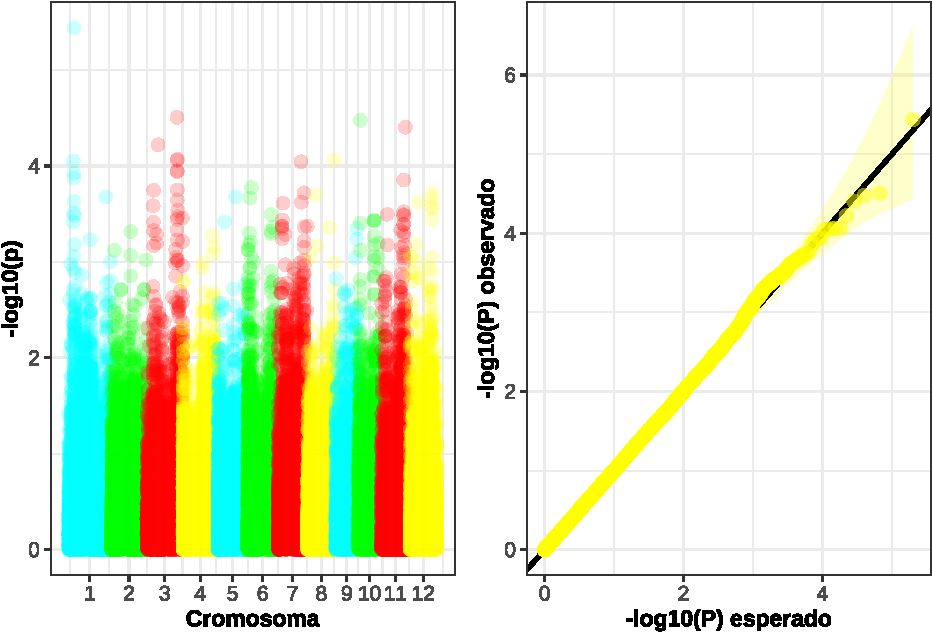
\includegraphics[width=1\linewidth]{figures/gwas} \end{center}

\hypertarget{matriz-de-parentesco-combinada}{%
\section{Matriz de parentesco combinada}\label{matriz-de-parentesco-combinada}}

\begin{center}\includegraphics[width=1\linewidth]{figures/map_H_Molcoanc} \end{center}

\hypertarget{habilidad-predictiva}{%
\section{Habilidad predictiva}\label{habilidad-predictiva}}

\captionsetup[table]{labelformat=empty,skip=1pt}
\begin{longtable}{crrrr}
\caption*{
{\large Pedirí 1} \\ 
{\small 751 individuos en total}
} \\ 
\toprule
 & \multicolumn{2}{c}{Bayesiano} & \multicolumn{2}{c}{REML} \\ 
 \cmidrule(lr){2-3} \cmidrule(lr){4-5}
Genotipados & Media & Desvío & Media & Desvíó \\ 
\midrule
\multicolumn{1}{l}{Densidad 0} \\ 
\midrule
0 & 0.515 & 0.061 & 0.513 & 0.055 \\ 
\midrule
\multicolumn{1}{l}{Densidad 1.000} \\ 
\midrule
148 & 0.483 & 0.051 & 0.464 & 0.062 \\ 
298 & 0.447 & 0.028 & 0.438 & 0.030 \\ 
451 & 0.493 & 0.002 & 0.495 & 0.000 \\ 
\midrule
\multicolumn{1}{l}{Densidad 10.000} \\ 
\midrule
148 & 0.490 & 0.054 & 0.479 & 0.063 \\ 
298 & 0.520 & 0.032 & 0.515 & 0.035 \\ 
451 & 0.586 & 0.002 & 0.585 & 0.000 \\ 
\midrule
\multicolumn{1}{l}{Densidad 100.000} \\ 
\midrule
148 & 0.496 & 0.056 & 0.482 & 0.064 \\ 
298 & 0.536 & 0.031 & 0.529 & 0.035 \\ 
451 & 0.581 & 0.002 & 0.580 & 0.000 \\ 
 \bottomrule
\end{longtable}
\captionsetup[table]{labelformat=empty,skip=1pt}
\begin{longtable}{crrrr}
\caption*{
{\large Pedirí 2} \\ 
{\small 1661 individuos en total}
} \\ 
\toprule
 & \multicolumn{2}{c}{Bayesiano} & \multicolumn{2}{c}{REML} \\ 
 \cmidrule(lr){2-3} \cmidrule(lr){4-5}
Genotipados & Media & Desvío & Media & Desvíó \\ 
\midrule
\multicolumn{1}{l}{Densidad 0} \\ 
\midrule
0 & 0.506 & 0.058 & 0.515 & 0.051 \\ 
\midrule
\multicolumn{1}{l}{Densidad 1.000} \\ 
\midrule
148 & 0.479 & 0.060 & 0.477 & 0.065 \\ 
298 & 0.454 & 0.024 & 0.454 & 0.026 \\ 
451 & 0.490 & 0.003 & 0.495 & 0.000 \\ 
\midrule
\multicolumn{1}{l}{Densidad 10.000} \\ 
\midrule
148 & 0.483 & 0.067 & 0.479 & 0.069 \\ 
298 & 0.539 & 0.024 & 0.538 & 0.025 \\ 
451 & 0.584 & 0.003 & 0.585 & 0.000 \\ 
\midrule
\multicolumn{1}{l}{Densidad 100.000} \\ 
\midrule
148 & 0.483 & 0.067 & 0.482 & 0.070 \\ 
298 & 0.550 & 0.023 & 0.552 & 0.025 \\ 
451 & 0.579 & 0.002 & 0.580 & 0.000 \\ 
 \bottomrule
\end{longtable}
\captionsetup[table]{labelformat=empty,skip=1pt}
\begin{longtable}{crrrr}
\caption*{
{\large Pedirí 3} \\ 
{\small 2451 individuos en total}
} \\ 
\toprule
 & \multicolumn{2}{c}{Bayesiano} & \multicolumn{2}{c}{REML} \\ 
 \cmidrule(lr){2-3} \cmidrule(lr){4-5}
Genotipados & Media & Desvío & Media & Desvíó \\ 
\midrule
\multicolumn{1}{l}{Densidad 0} \\ 
\midrule
0 & 0.495 & 0.059 & 0.509 & 0.054 \\ 
\midrule
\multicolumn{1}{l}{Densidad 1.000} \\ 
\midrule
148 & 0.484 & 0.051 & 0.480 & 0.058 \\ 
298 & 0.439 & 0.036 & 0.441 & 0.036 \\ 
451 & 0.490 & 0.002 & 0.495 & 0.000 \\ 
\midrule
\multicolumn{1}{l}{Densidad 10.000} \\ 
\midrule
148 & 0.491 & 0.055 & 0.488 & 0.057 \\ 
298 & 0.524 & 0.031 & 0.525 & 0.031 \\ 
451 & 0.583 & 0.005 & 0.585 & 0.000 \\ 
\midrule
\multicolumn{1}{l}{Densidad 100.000} \\ 
\midrule
148 & 0.494 & 0.055 & 0.492 & 0.058 \\ 
298 & 0.538 & 0.033 & 0.540 & 0.031 \\ 
451 & 0.578 & 0.002 & 0.580 & 0.000 \\ 
 \bottomrule
\end{longtable}

\hypertarget{habilidad-predictiva-1}{%
\section{Habilidad predictiva}\label{habilidad-predictiva-1}}

\captionsetup[table]{labelformat=empty,skip=1pt}
\begin{longtable}{lrrrr}
\caption*{
{\large Pedirí 1} \\ 
{\small 2061 individuos en total}
} \\ 
\toprule
 & \multicolumn{2}{c}{F2} & \multicolumn{2}{c}{F3} \\ 
 \cmidrule(lr){2-3} \cmidrule(lr){4-5}
Genotipados & Media & Desvío & Media & Desvío \\ 
\midrule
\multicolumn{1}{l}{Densidad 0} \\ 
\midrule
Ninguno & 0.577 & 0.092 & 0.562 & 0.086 \\ 
\midrule
\multicolumn{1}{l}{Densidad 1.000} \\ 
\midrule
F0-F1-F2-F3 & 0.597 & 0.072 & 0.565 & 0.076 \\ 
F1-F2 & 0.582 & 0.093 & 0.566 & 0.091 \\ 
F2 & 0.580 & 0.094 & 0.565 & 0.091 \\ 
\midrule
\multicolumn{1}{l}{Densidad 10.000} \\ 
\midrule
F0-F1-F2-F3 & 0.627 & 0.060 & 0.610 & 0.064 \\ 
F1-F2 & 0.583 & 0.093 & 0.568 & 0.089 \\ 
F2 & 0.582 & 0.098 & 0.567 & 0.090 \\ 
\midrule
\multicolumn{1}{l}{Densidad 100.000} \\ 
\midrule
F0-F1-F2-F3 & 0.629 & 0.061 & 0.618 & 0.065 \\ 
F1-F2 & 0.583 & 0.093 & 0.569 & 0.088 \\ 
F2 & 0.581 & 0.097 & 0.568 & 0.090 \\ 
 \bottomrule
\end{longtable}
\captionsetup[table]{labelformat=empty,skip=1pt}
\begin{longtable}{lrrrr}
\caption*{
{\large Pedirí 2} \\ 
{\small 2071 individuos en total}
} \\ 
\toprule
 & \multicolumn{2}{c}{F2} & \multicolumn{2}{c}{F3} \\ 
 \cmidrule(lr){2-3} \cmidrule(lr){4-5}
Genotipados & Media & Desvío & Media & Desvío \\ 
\midrule
\multicolumn{1}{l}{Densidad 0} \\ 
\midrule
Ninguno & 0.574 & 0.095 & 0.560 & 0.091 \\ 
\midrule
\multicolumn{1}{l}{Densidad 1.000} \\ 
\midrule
F0-F1-F2-F3 & 0.592 & 0.092 & 0.574 & 0.096 \\ 
F1-F2 & 0.589 & 0.093 & 0.573 & 0.091 \\ 
F2 & 0.589 & 0.094 & 0.574 & 0.091 \\ 
\midrule
\multicolumn{1}{l}{Densidad 10.000} \\ 
\midrule
F0-F1-F2-F3 & 0.632 & 0.080 & 0.623 & 0.079 \\ 
F1-F2 & 0.590 & 0.092 & 0.577 & 0.092 \\ 
F2 & 0.590 & 0.092 & 0.576 & 0.092 \\ 
\midrule
\multicolumn{1}{l}{Densidad 100.000} \\ 
\midrule
F0-F1-F2-F3 & 0.635 & 0.079 & 0.627 & 0.081 \\ 
F1-F2 & 0.591 & 0.094 & 0.576 & 0.092 \\ 
F2 & 0.590 & 0.093 & 0.576 & 0.092 \\ 
 \bottomrule
\end{longtable}
\captionsetup[table]{labelformat=empty,skip=1pt}
\begin{longtable}{lrrrr}
\caption*{
{\large Pedirí 3} \\ 
{\small 2091 individuos en total}
} \\ 
\toprule
 & \multicolumn{2}{c}{F2} & \multicolumn{2}{c}{F3} \\ 
 \cmidrule(lr){2-3} \cmidrule(lr){4-5}
Genotipados & Media & Desvío & Media & Desvío \\ 
\midrule
\multicolumn{1}{l}{Densidad 0} \\ 
\midrule
Ninguno & 0.582 & 0.053 & 0.558 & 0.042 \\ 
\midrule
\multicolumn{1}{l}{Densidad 1.000} \\ 
\midrule
F0-F1-F2-F3 & 0.616 & 0.047 & 0.586 & 0.041 \\ 
F1-F2 & 0.603 & 0.051 & 0.578 & 0.051 \\ 
F2 & 0.601 & 0.051 & 0.576 & 0.050 \\ 
\midrule
\multicolumn{1}{l}{Densidad 10.000} \\ 
\midrule
F0-F1-F2-F3 & 0.646 & 0.039 & 0.626 & 0.035 \\ 
F1-F2 & 0.607 & 0.053 & 0.583 & 0.048 \\ 
F2 & 0.605 & 0.053 & 0.579 & 0.049 \\ 
\midrule
\multicolumn{1}{l}{Densidad 100.000} \\ 
\midrule
F0-F1-F2-F3 & 0.652 & 0.040 & 0.632 & 0.031 \\ 
F1-F2 & 0.607 & 0.052 & 0.583 & 0.048 \\ 
F2 & 0.607 & 0.052 & 0.581 & 0.049 \\ 
 \bottomrule
\end{longtable}
\captionsetup[table]{labelformat=empty,skip=1pt}
\begin{longtable}{lrrrr}
\caption*{
{\large Pedirí 4} \\ 
{\small 2131 individuos en total}
} \\ 
\toprule
 & \multicolumn{2}{c}{F2} & \multicolumn{2}{c}{F3} \\ 
 \cmidrule(lr){2-3} \cmidrule(lr){4-5}
Genotipados & Media & Desvío & Media & Desvío \\ 
\midrule
\multicolumn{1}{l}{Densidad 0} \\ 
\midrule
Ninguno & 0.556 & 0.047 & 0.538 & 0.044 \\ 
\midrule
\multicolumn{1}{l}{Densidad 1.000} \\ 
\midrule
F0-F1-F2-F3 & 0.596 & 0.041 & 0.569 & 0.053 \\ 
F1-F2 & 0.579 & 0.050 & 0.563 & 0.053 \\ 
F2 & 0.580 & 0.052 & 0.561 & 0.054 \\ 
\midrule
\multicolumn{1}{l}{Densidad 10.000} \\ 
\midrule
F0-F1-F2-F3 & 0.624 & 0.036 & 0.609 & 0.038 \\ 
F1-F2 & 0.586 & 0.049 & 0.570 & 0.049 \\ 
F2 & 0.586 & 0.047 & 0.568 & 0.050 \\ 
\midrule
\multicolumn{1}{l}{Densidad 100.000} \\ 
\midrule
F0-F1-F2-F3 & 0.628 & 0.034 & 0.615 & 0.038 \\ 
F1-F2 & 0.586 & 0.050 & 0.571 & 0.050 \\ 
F2 & 0.585 & 0.050 & 0.569 & 0.051 \\ 
 \bottomrule
\end{longtable}

\backmatter

\hypertarget{bibliografuxeda}{%
\chapter*{Bibliografía}\label{bibliografuxeda}}
\addcontentsline{toc}{chapter}{Bibliografía}

\markboth{\MakeUppercase{Bibliography}}{} % have to explicitly state what to put in the heading (bug in bookdown?)
%format the references so they have a hanging indent. Remove these (and the \endgroup command) if you want regular indentation.
\begingroup
\hspace{\parindent}
\setlength{\parindent}{-0.25in}
\setlength{\leftskip}{0.25in}
\setlength{\parskip}{0pt}

\hypertarget{refs}{}
\leavevmode\hypertarget{ref-cite:33}{}%
Ahmadi, N., J. Bartholomé, T. V. Cao, y C. Grenier. 2020a. \emph{Quantitative genetics, genomics and plant breeding}. 2nd edition. \url{https://doi.org/10.1079/9781789240214.0243}.

\leavevmode\hypertarget{ref-cite:45}{}%
Ahmadi, N., J. Bartholomé, T V. Cao, y C. Grenier. 2020b. \emph{Genomic selection in rice: empirical results and implications for breeding}. 2nd edition. CAB International.

\leavevmode\hypertarget{ref-cite:58}{}%
Bartholomé, J., P. Thathapalli-Prakash, y J. N. Cobb. 2021. \emph{Genomic prediction: progress and perspectives for rice improvement}. \url{https://doi.org/10.48550/arXiv.2109.14781}.

\leavevmode\hypertarget{ref-cite:21}{}%
Blasco, A. 2021. \emph{Mejora genética animal}. 1st edition. EDITORIAL SÍNTESIS, S. A.

\leavevmode\hypertarget{ref-cite:3}{}%
Blasco, A., y M. A. Toro. 2014. «A short critical history of the application of genomics to animal breeding». \emph{Livestock Science} 166: 4-9.

\leavevmode\hypertarget{ref-cite:57}{}%
Breseghello, F. 2013. «Traditional and modern plant breeding methods with wxamples in rice (Oryza sativa L.)». \emph{Journal of Agricultural and Food Chemistry} 61: 8277-86. \url{https://doi.org/10.1021/jf305531j}.

\leavevmode\hypertarget{ref-cite:51}{}%
Caamal-Pat, D, P. Pérez-Rodríguez, J. Crossa, C. Velasco-Cruz, S. Pérez-Elizalde, y M. Vázquez-Peña. 2021. «lme4GS: An R-package for genomic selection». \emph{Genetics} 12. \url{https://doi.org/10.3389/fgene.2021.680569}.

\leavevmode\hypertarget{ref-cite:42}{}%
Caligari, P. D. S., y J. Brown. 2017. \emph{Plant breeding, practice}. 2nd edition. Vol. 2. Elsevier Ltd. \url{https://doi.org/10.1016/B978-0-12-394807-6.00195-7}.

\leavevmode\hypertarget{ref-cite:64}{}%
Cappetta, E., G. Andolfo, A. Di Matteo, A. Barone, L Frusciante, y M. R. Ercolano. 2020. «Accelerating tomato breeding by exploiting genomic selection approaches». \emph{Plants} 9 (9). \url{https://doi.org/10.3390/plants9091236}.

\leavevmode\hypertarget{ref-cite:48}{}%
Cros, D., L. Sánchez, B. Cochard, P. Samper, M. Denis, J. M. Bouvet, y J. Fernández. 2014. «Estimation of genealogical coancestry in plant species using a pedigree reconstruction algorithm and application to an oil palm breeding population». \emph{Theoretical and Applied Genetics} 127: 981-94. \url{https://doi.org/10.1007/s00122-014-2273-3}.

\leavevmode\hypertarget{ref-cite:37}{}%
Crossa, J., P. Pérez-Rodríguez, J. Cuevas, O. Montesinos-López, D. Jarquín, G. de los Campos, J. Burgueño, et~al. 2017. «Genomic selection in plant breeding: methods, models, and perspectives». \emph{Trends in Plant Science}, 961-75. \url{https://doi.org/10.1016/j.tplants.2017.08.011}.

\leavevmode\hypertarget{ref-cite:59}{}%
Dekkers, J., y F. Hospital. 2002. «The use of molecular genetics in the improvement of agricultural populations». \emph{Nature Reviews Genetics} 3: 22-32. \url{https://doi.org/10.1038/nrg701}.

\leavevmode\hypertarget{ref-cite:31}{}%
de los Campos, G., J. H. Hickey, R. Pong-Wong, H. D. Daetwyler, y M. P. L. Calus. 2013. «Whole-genome regression and prediction methods applied to plant and animal breeding». \emph{Genetics} 193: 327-45. \url{https://doi.org/10.1534/genetics.112.143313}.

\leavevmode\hypertarget{ref-cite:10}{}%
Desta, Z. A., y R. Ortiz. 2014. «Genomic selection: genome-wide prediction in plant improvement». \emph{Trends in Plant Science} 19 (9): 592-601.

\leavevmode\hypertarget{ref-cite:24}{}%
Fernández, J., y M. Toro. 2006. «A new method to estimate relatedness from molecular markers». \emph{Molecular Ecology} 15: 1657-67.

\leavevmode\hypertarget{ref-cite:28}{}%
Freeman, A. E. 1991. «C. R. Henderson: contributions to the dairy industry». \emph{Journal of Dairy Science} 74 (11): 4045-51. \url{https://doi.org/10.3168/jds.S0022-0302(91)78600-1}.

\leavevmode\hypertarget{ref-cite:61}{}%
Fukuoka, S., K. Ebana, T. Yamamoto, y M. Yano. 2010. «Integration of genomics into rice breeding». \emph{Rice} 3: 131-37. \url{https://doi.org/10.1007/s12284-010-9044-9}.

\leavevmode\hypertarget{ref-cite:65}{}%
Grenier, C., T. V. Cao, Y. Ospina, C. Quintero, M. H. Châtel, J. Tohme, B. Courtois, y N. Ahmadi. 2015. «Accuracy of genomic selection in a rice synthetic population developed for recurrent selection breeding». \emph{PLoS ONE} 10 (8). \url{https://doi.org/10.1371/journal.pone.0136594}.

\leavevmode\hypertarget{ref-cite:62}{}%
Guimarães, E. P. 2009. \emph{Rice Breeding}. \url{https://doi.org/10.1007/978-0-387-72297-9/_2}.

\leavevmode\hypertarget{ref-cite:41}{}%
Henderson, C. R. 1975. «Best linear unbiased estimation and prediction under a selection model». \emph{Biometrics} 31: 423-47.

\leavevmode\hypertarget{ref-cite:67}{}%
---------. 1986. \emph{Applications of linear models in animal breeding}. 2nd edition.

\leavevmode\hypertarget{ref-cite:44}{}%
Hickey, J. M., T. Chiurugwi, I. Mackay, W. Powell, y Implementing Genomic Selection in CGIAR Breeding Programs Workshop Participants. 2017. «Genomic prediction unifies animal and plant breeding programs to form platforms for biological discovery». \emph{Nature Genetics} 49 (9): 1297-1303. \url{https://doi.org/10.1038/ng.3920}.

\leavevmode\hypertarget{ref-cite:43}{}%
Holland, J. B. 2014. \emph{Breeding: plants, modern}. Vol. 2. Elsevier Inc. \url{https://doi.org/10.1016/B978-0-444-52512-3.00226-6}.

\leavevmode\hypertarget{ref-cite:20}{}%
Imai, A., T. Kuniga, T. Yoshioka, K. Nonaka, N. Mitani, H. Fukamachi, N. Hiehata, M. Yamamoto, y T. Hayashi. 2019. «Single-step genomic prediction of fruit-quality traits using phenotypic records of non-genotyped relatives in citrus». \emph{PLoS ONE} 14 (8). \url{https://doi.org/10.1371/journal.pone.0221880}.

\leavevmode\hypertarget{ref-cite:11}{}%
Jurcic, E. J., P. V. Villalba, P. S. Pathauer, D. A. Palazzini, G. P. J. Oberschelp, L. Harrand, M. N. Garcia, et~al. 2021. «Single-setp genomic prediction of Eucalyptus dunni using different identity-by-descent and identity-by-state relationship matrices». \emph{Heredity} 127: 176-89.

\leavevmode\hypertarget{ref-cite:32}{}%
Kyselova, J., L. Tichý, y K. Jochová. 2021. «The role of molecular genetics in animal breeding: a minireview». \emph{Czech Journal of Animal Science} 66 (4): 107-11. \url{https://doi.org/10.17221/251/2020-CJAS}.

\leavevmode\hypertarget{ref-cite:17}{}%
Legarra, A., I. Aguilar, y I. Misztal. 2009. «A relationship matrix including full pedigree and genomic information». \emph{Journal of Dairy Science} 92: 4656-63. \url{https://doi.org/10.3168/jds.2009-2061}.

\leavevmode\hypertarget{ref-cite:15}{}%
Legarra, A., O. F. Christensen, I. Aguilar, y I. Misztal. 2014. «Single Step, a general approach for genomic selection». \emph{Livestock Science}. \url{https://doi.org/10.1016/j.livsci.2014.04.029}.

\leavevmode\hypertarget{ref-cite:30}{}%
Legarra, A., D. Lourenco, y Z. G. Vitezica. 2018. \emph{Bases for genomic prediction}.

\leavevmode\hypertarget{ref-cite:22}{}%
Lourenco, D., A. Legarra, S. Tsuruta, Y. Masuda, I. Aguilar, y I. Misztal. 2020. «Single-step genomic evaluations from theory to practice: using SNP chips and sequence data in BLUPF90». \emph{Genes} 11: 790. \url{https://doi.org/doi:10.3390/genes11070790}.

\leavevmode\hypertarget{ref-cite:38}{}%
Medina, C. A., H. Kaur, I. Ray, y L. X. Yu. 2021. «Strategies to Increase Prediction Accuracy in Genomic Selection of Complex Traits in Alfalfa (Medicago sativa L.)». \emph{Cells} 10 (12). \url{https://doi.org/10.3390/cells10123372}.

\leavevmode\hypertarget{ref-cite:8}{}%
Meuwissen, T. H. E., B. J. Hayes, y M. E. Goddard. 2001. «Prediction of Total Genetic Value Using Genome-Wide Dense Marker Maps». \emph{Genetics} 157: 1819-29.

\leavevmode\hypertarget{ref-cite:14}{}%
Misztal, I., S. E. Aggrrey, y W. M. Muir. 2012. «Experiences with a single-step genome evaluation». \emph{Poultry Science} 92: 2530-4.

\leavevmode\hypertarget{ref-cite:16}{}%
Misztal, I., A. Legarra, y I. Aguilar. 2009. «Computing procedures for genetic evaluation including phenotypic, full pedigree, and genomic information». \emph{Journal of Dairy Science} 92: 4648-55. \url{https://doi.org/10.3168/jds.2009-2064}.

\leavevmode\hypertarget{ref-cite:18}{}%
Misztal, I., D. Lourenco, y A. Legarra. 2020. «Current status of genomic evaluation». \emph{Journal of Animal Science} 98 (4): 1-14. \url{https://doi.org/10.1093/jas/skaa101}.

\leavevmode\hypertarget{ref-cite:68}{}%
Morais-Júnior, O. P., F. Breseghello, J. Batista-Duarte, A. S. G. Coelho, T. C. O. Borba, J. T. Aguiar, P. C. F. Neves, y O. P. Morais. 2018. «Assessing prediction models for different traits in a rice population derived from a recurrent selection program». \emph{Crop Science} 58: 1-13. \url{https://doi.org/10.2135/cropsci2018.02.0087}.

\leavevmode\hypertarget{ref-cite:6}{}%
Nakaya, A., y S. N. Isobe. 2012. «Will genomic selection be a practical method for plant breeding?» \emph{Annals of Botany} 110: 1303-16.

\leavevmode\hypertarget{ref-cite:2}{}%
Nelson, R. M., M. E. Pettersson, y Ö. Carlborg. 2012. «A century after Fisher: time for a new paradigm in quantitative genetics». \emph{Trends in Genetics} 29 (9): 669-76.

\leavevmode\hypertarget{ref-cite:47}{}%
Pérez-Enciso, M., L. Ramírez-Ayala, y L. M. Zingaretti. 2020. «SeqBreed: a python tool to evaluate genomic prediction in complex scenarios». \emph{Genetion Selection Evolution} 52 (7). \url{https://doi.org/10.1186/s12711-020-0530-2}.

\leavevmode\hypertarget{ref-cite:19}{}%
Pérez-Rodríguez, P., J. Crossa, J. Rutkoski, J. Poland, R. Singh, A. Legarra, E. Autrique, J. Burgueño G. de los Campos, y S. Dreisigacker. 2017. «Single-step genomic and pedigree genotype x environment interaction models for predicting wheat lines in international environments». \emph{Plant Genome} 10 (2). \url{https://doi.org/10.3835/plantgenome2016.09.0089}.

\leavevmode\hypertarget{ref-cite:50}{}%
Pérez-Rodríguez, P., y G. de los Campos. 2014. «Genome-wide regression and prediction with the BGLR statistical package». \emph{Genetics} 198 (2): 483-95. \url{https://www.ncbi.nlm.nih.gov/pmc/articles/PMC4196607/}.

\leavevmode\hypertarget{ref-cite:49}{}%
Purcell, S., B. Neale, K. Todd-Brown, L. Thomas, M. A. R. Ferreira, D. Bender, J. Maller, et~al. 2007. «Plink: a toolset for whole-genome association and population-based linkage analysis». \emph{American Journal of Human Genetics} 81: 981-94. \url{http://pngu.mgh.harvard.edu/purcell/plink/}.

\leavevmode\hypertarget{ref-cite:52}{}%
R Core Team. 2020. \emph{R: A Language and Environment for Statistical Computing}. Vienna, Austria: R Foundation for Statistical Computing. \url{https://www.R-project.org/}.

\leavevmode\hypertarget{ref-cite:63}{}%
Robertsen, C. D., R. L. Hjortshøj, y L. L. Janss. 2019. «Genomic selection in cereal breeding». \emph{Agronomy} 9: 95. \url{https://doi.org/10.3390/agronomy9020095}.

\leavevmode\hypertarget{ref-cite:27}{}%
Schaeffer, L. R. 1991. «C. R. Henderson: contributions to predicting genetic merit». \emph{Journal of Dairy Science} 74 (11): 4052-66. \url{https://doi.org/10.3168/jds.S0022-0302(91)78601-3}.

\leavevmode\hypertarget{ref-cite:29}{}%
Searle, S. R. 1991. «C. R. Henderson, the statistician; and his contributions to variance components estimation». \emph{Journal of Dairy Science} 74 (11): 4035-44. \url{https://doi.org/10.3168/jds.S0022-0302(91)78599-8}.

\leavevmode\hypertarget{ref-cite:34}{}%
Tan, C., C. Bian, D. Yang, N. Li, Z. Wu, y X. Hu. 2017. «Application of genomic selection in farm animal breeding». \emph{Hereditas} 39 (11): 1033-45. \url{https://doi.org/10.16288/j.yczz.17-286}.

\leavevmode\hypertarget{ref-cite:7}{}%
Tong, H., y Z. Nikoloski. 2021. «Machine learning approaches for crop improvement: leveraging phenotypic and genotypic big data». \emph{Journal of Plant Physiology} 257: 153354. \url{https://doi.org/10.1016/j.jplph.2020.153354}.

\leavevmode\hypertarget{ref-cite:9}{}%
Turelli, M. 2017. «Prediction of Total Genetic Value Using Genome-Wide Dense Marker Maps». \emph{Theoretical Population Biology} 118: 46-49.

\leavevmode\hypertarget{ref-cite:39}{}%
VanRaden, P. M. 2007. «Efficient methods to compute genomic predictions». \emph{Journal of Dairy Science} 91: 4414-23.

\leavevmode\hypertarget{ref-cite:53}{}%
Van-Rossum, G., y Jr. F. L Drake. 1995. \emph{Python reference manual}. Centrum voor Wiskunde en Informatica Amsterdam.

\leavevmode\hypertarget{ref-cite:26}{}%
Vourlaki, I., R. Castanera, S. Ramos-Onsins, J. Casacuberta, y M. Pérez-Enciso. s.~f. «Transposable element polymorphisms improve prediction of complex agronomic traits in rice». \emph{Frontiers in Plant Science}.

\leavevmode\hypertarget{ref-cite:46}{}%
Wang, J., J. Crossa, y J. Gai. 2020. «Quantitative genetic studies with applications in plant breeding in the omics era». \emph{The Crop Journal} 8: 683-87. \url{https://doi.org/10.1016/j.cj.2020.09.001}.

\leavevmode\hypertarget{ref-cite:55}{}%
Wing, R. A., M. D. Purugganan, y Q. Zhang. 2018. «The rice genome revolution: from an ancient grain to Green Super Rice». \emph{Nature Reviews Genetics} 19: 505-17. \url{https://doi.org/10.1038/s41576-018-0024-z}.

\leavevmode\hypertarget{ref-cite:60}{}%
Xu, Y., K. Ma, Y. Zhao, X. Wang, K. Zhou, G. Yu, C. Li, et~al. 2021. «Genomic selection: a breakthrough technology in rice breeding». \emph{Nature Reviews Genetics} 9: 669-77. \url{https://doi.org/10.1016/j.cj.2021.03.008}.

\leavevmode\hypertarget{ref-cite:25}{}%
Xua, S., D. Zhub, y Q. Zhang. 2014. «Predicting hybrid performance in rice using genomic best linear unbiased prediction». \emph{Proceedings of the National Academy of Sciences of the United States of America} 111 (34): 12456-61. \url{https://doi.org/10.1073/pnas.1413750111}.

\leavevmode\hypertarget{ref-cite:54}{}%
Yang, J., S. H. Lee, M. E. Goddard, y P. M. Visscher. 2011. «GCTA: A Tool for Genome-wide Complex Trait Analysis». \emph{American Journal of Human Genetics} 88 (1): 76-82. \url{https://doi.org/10.1016/j.ajhg.2010.11.011}.

\endgroup

\hypertarget{agradecimientos}{%
\chapter*{Agradecimientos}\label{agradecimientos}}
\addcontentsline{toc}{chapter}{Agradecimientos}

\chaptermark{Acknowledgments}

\includegraphics{figures/uvalogo_regular_p_en.pdf}

\backmatter

\end{document}
